\chapter{Experiment}
Sensor:\\
Hokuyo UBG 04-LX - 2D scanning laser rangefinder. Measures range\\

Robot arm: \\
Kinova Jaco - can program to move with and record pose

Target object: \\
$0.1 \times 0.1$ m MDF cube, spray painted matte white

1. Collected measurements to model sensor noise for simulation\\
2. Collected measurements of moving cube + measured ground truth cube state - for testing observer with real world conditions

\section{Sensor Noise Characterisation} \label{sensor_noise}
	\subsection{Setup}
		\textbf{physical setup:}\\
		\textbf{measurement configurations:}\\
			-5cm increments from 0.25-1.75m\\
			-vary incidence angle: 0,20,40,60,80 degrees
		 
	\subsection{Results}
		\textbf{Error distribution:}
		Histograms (Figure \ref{fig:mean_hist}) - range error approximately normally distributed:
		\begin{figure}
		\centering
		  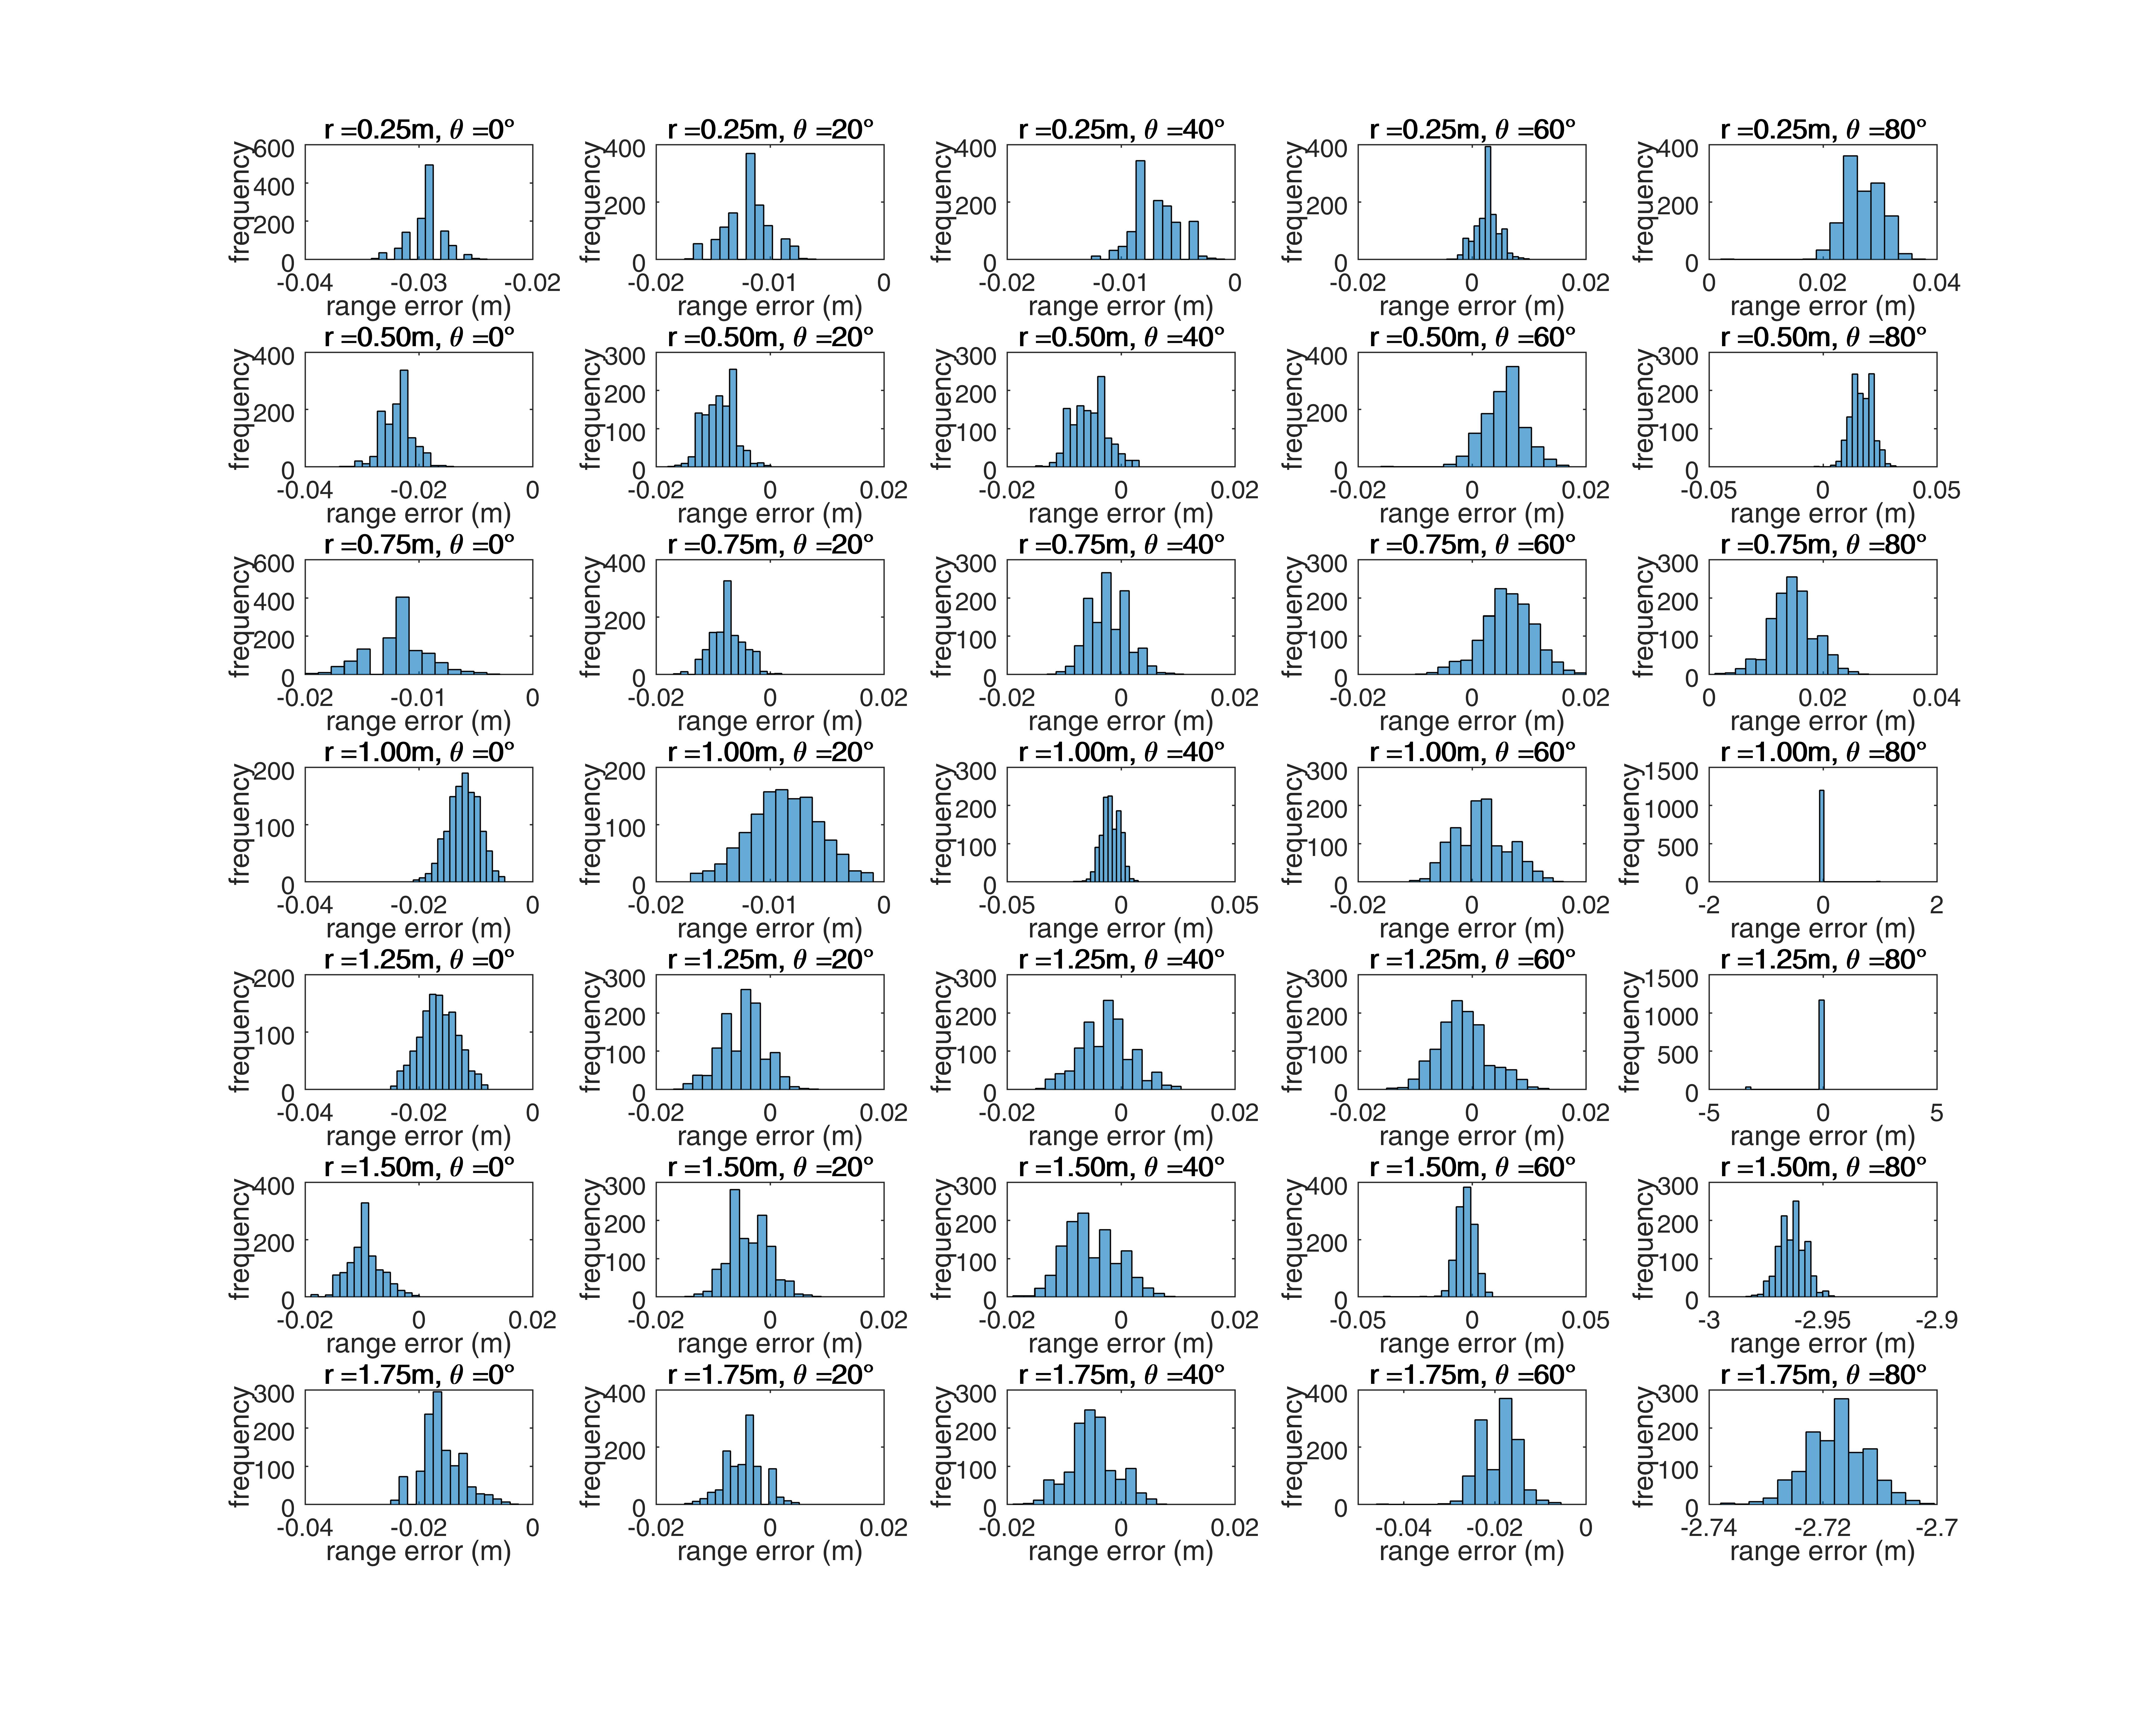
\includegraphics[width=1\textwidth,trim = 0mm 0mm 0mm 0mm,clip]{./Figures/range_error_histograms.jpg}
		  \caption{$r_{error}(r,\theta)$ approximately normally distributed}
		  \label{fig:mean_hist}
		\end{figure}
		
		Mean range error as function of (range,incidence angle) - Figure \ref{fig:mean_range_error}
		\begin{figure}
	  		\centering
	  		\subfigure[\label{fig:mean_range_error_outliers}]{
	  		\begin{minipage}[b]{0.45\columnwidth}
    			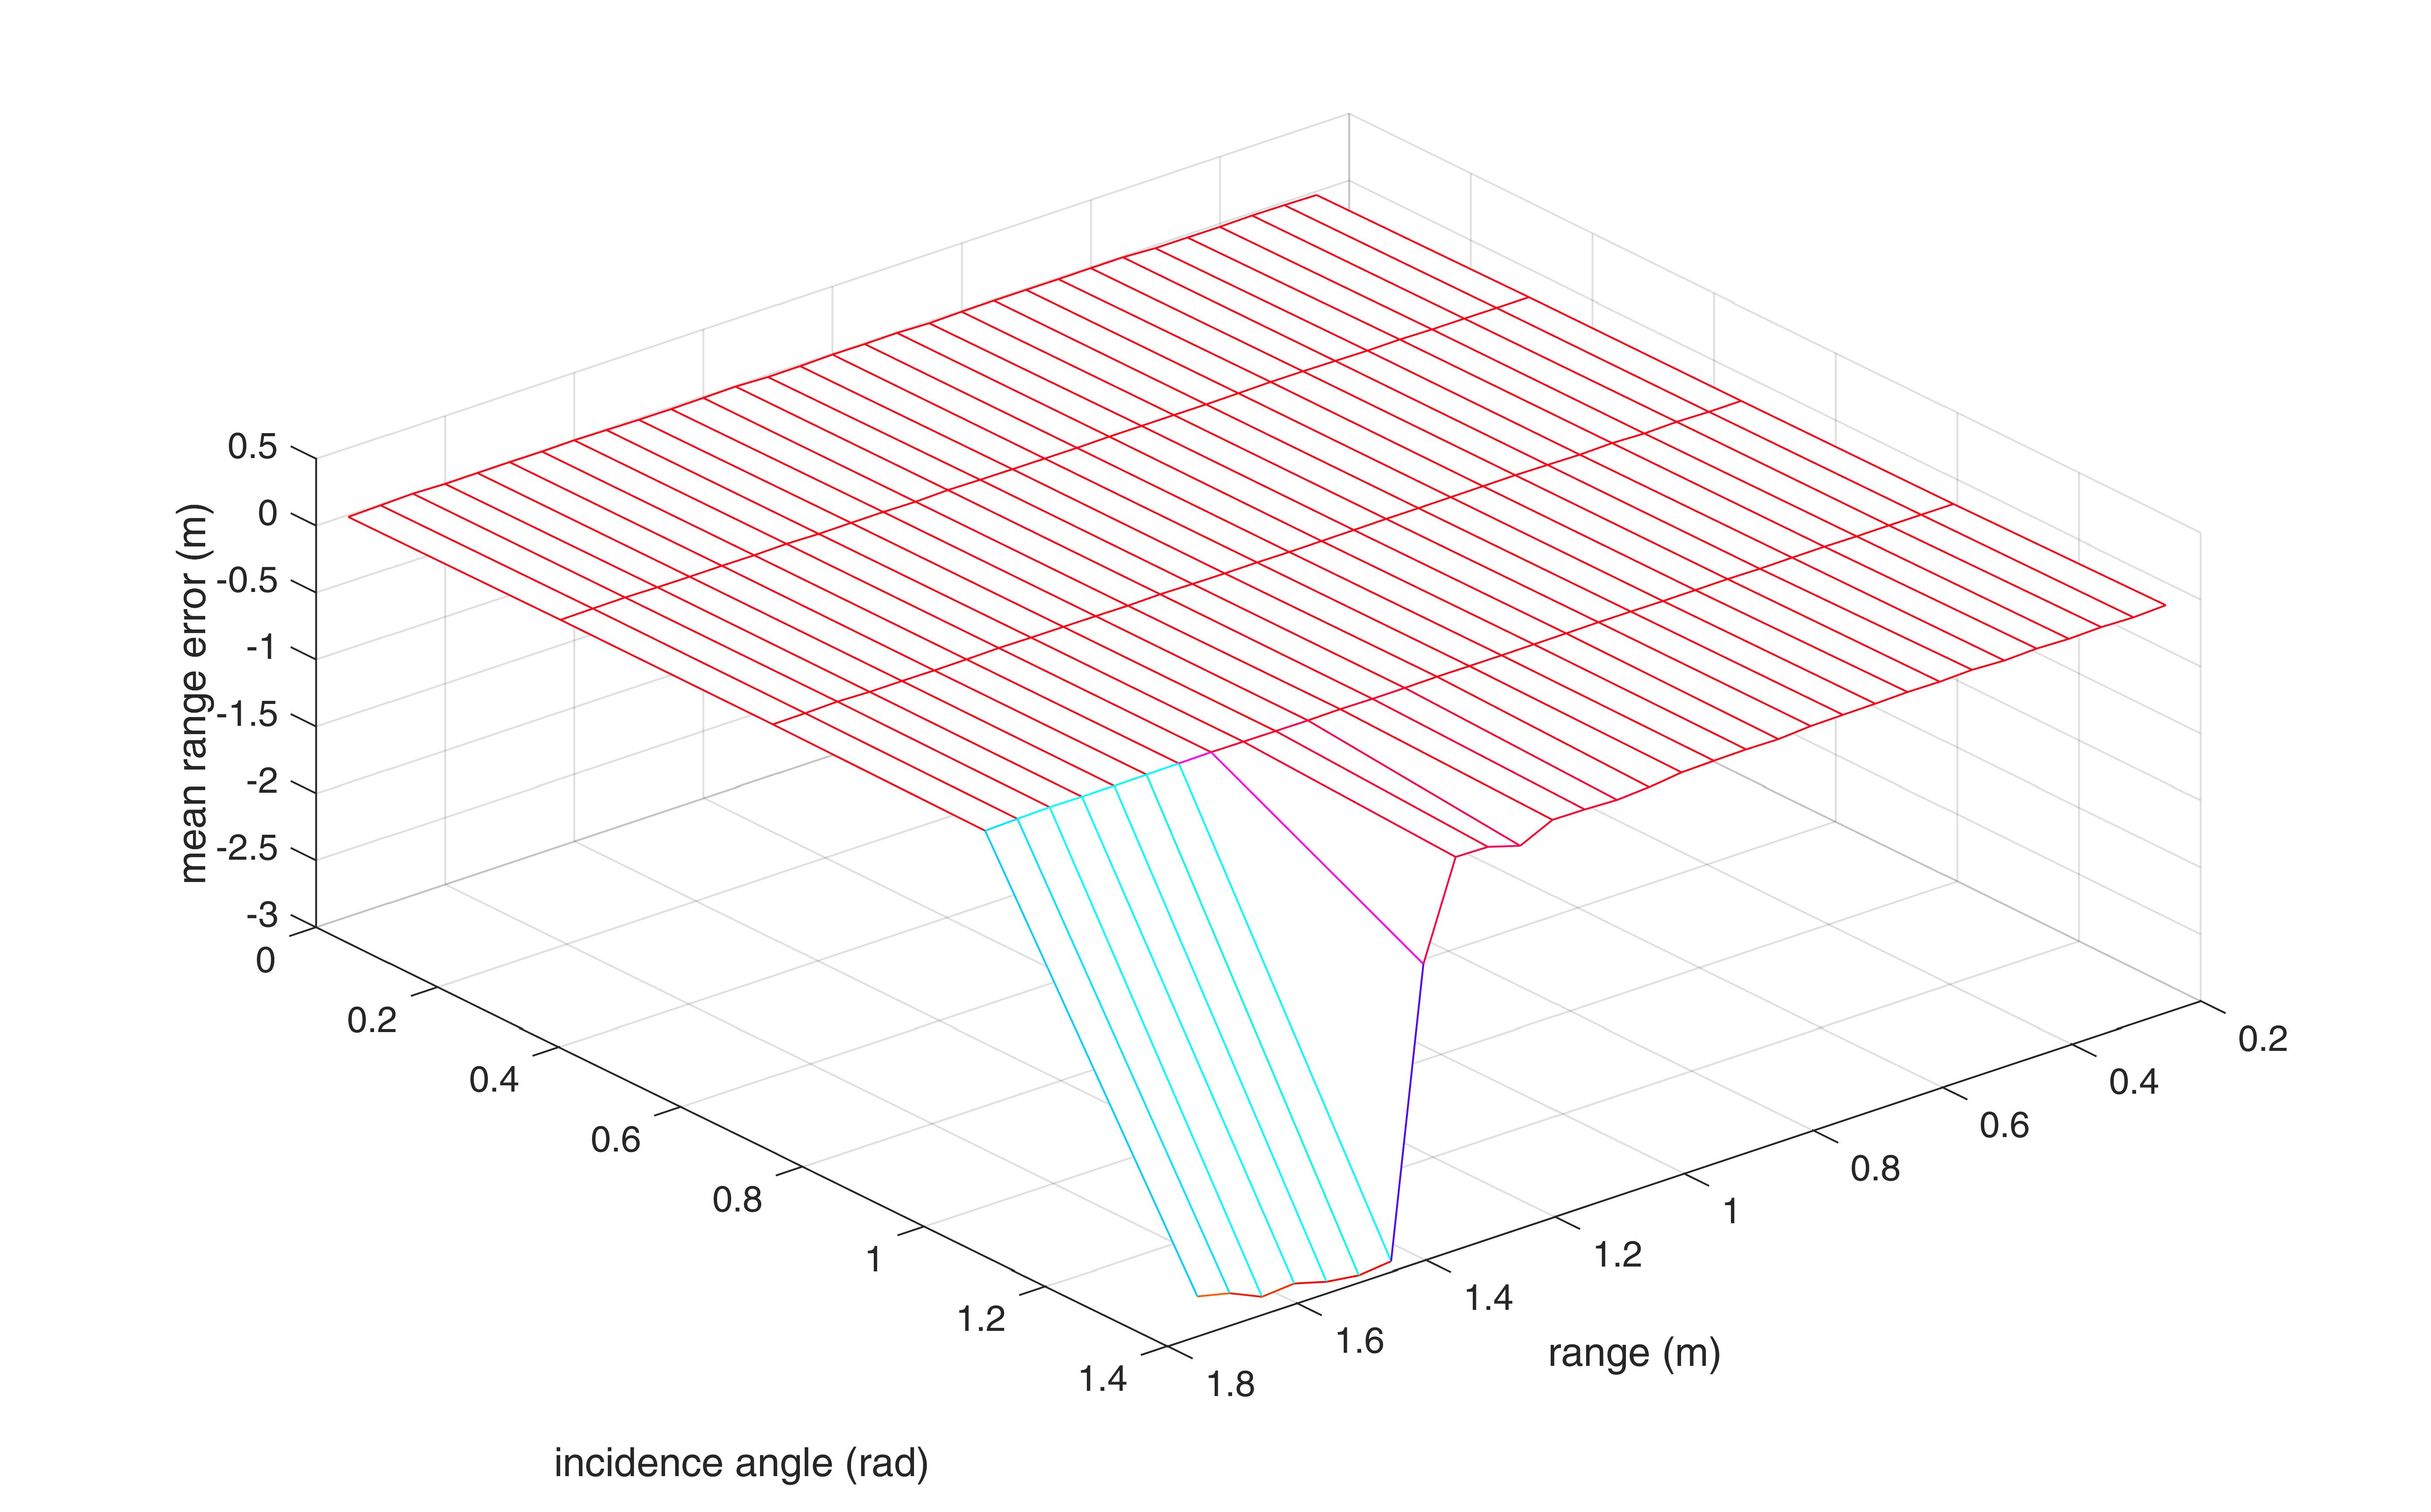
\includegraphics[width=1\textwidth,trim = 0mm 0mm 0mm 0mm,clip]{./Figures/noise_mean_range_error}\vspace*{0ex}
	  		\end{minipage}}
	  		\subfigure[\label{fig:mean_range_error_no_outliers}]{
	  		\begin{minipage}[b]{0.45\columnwidth}
    			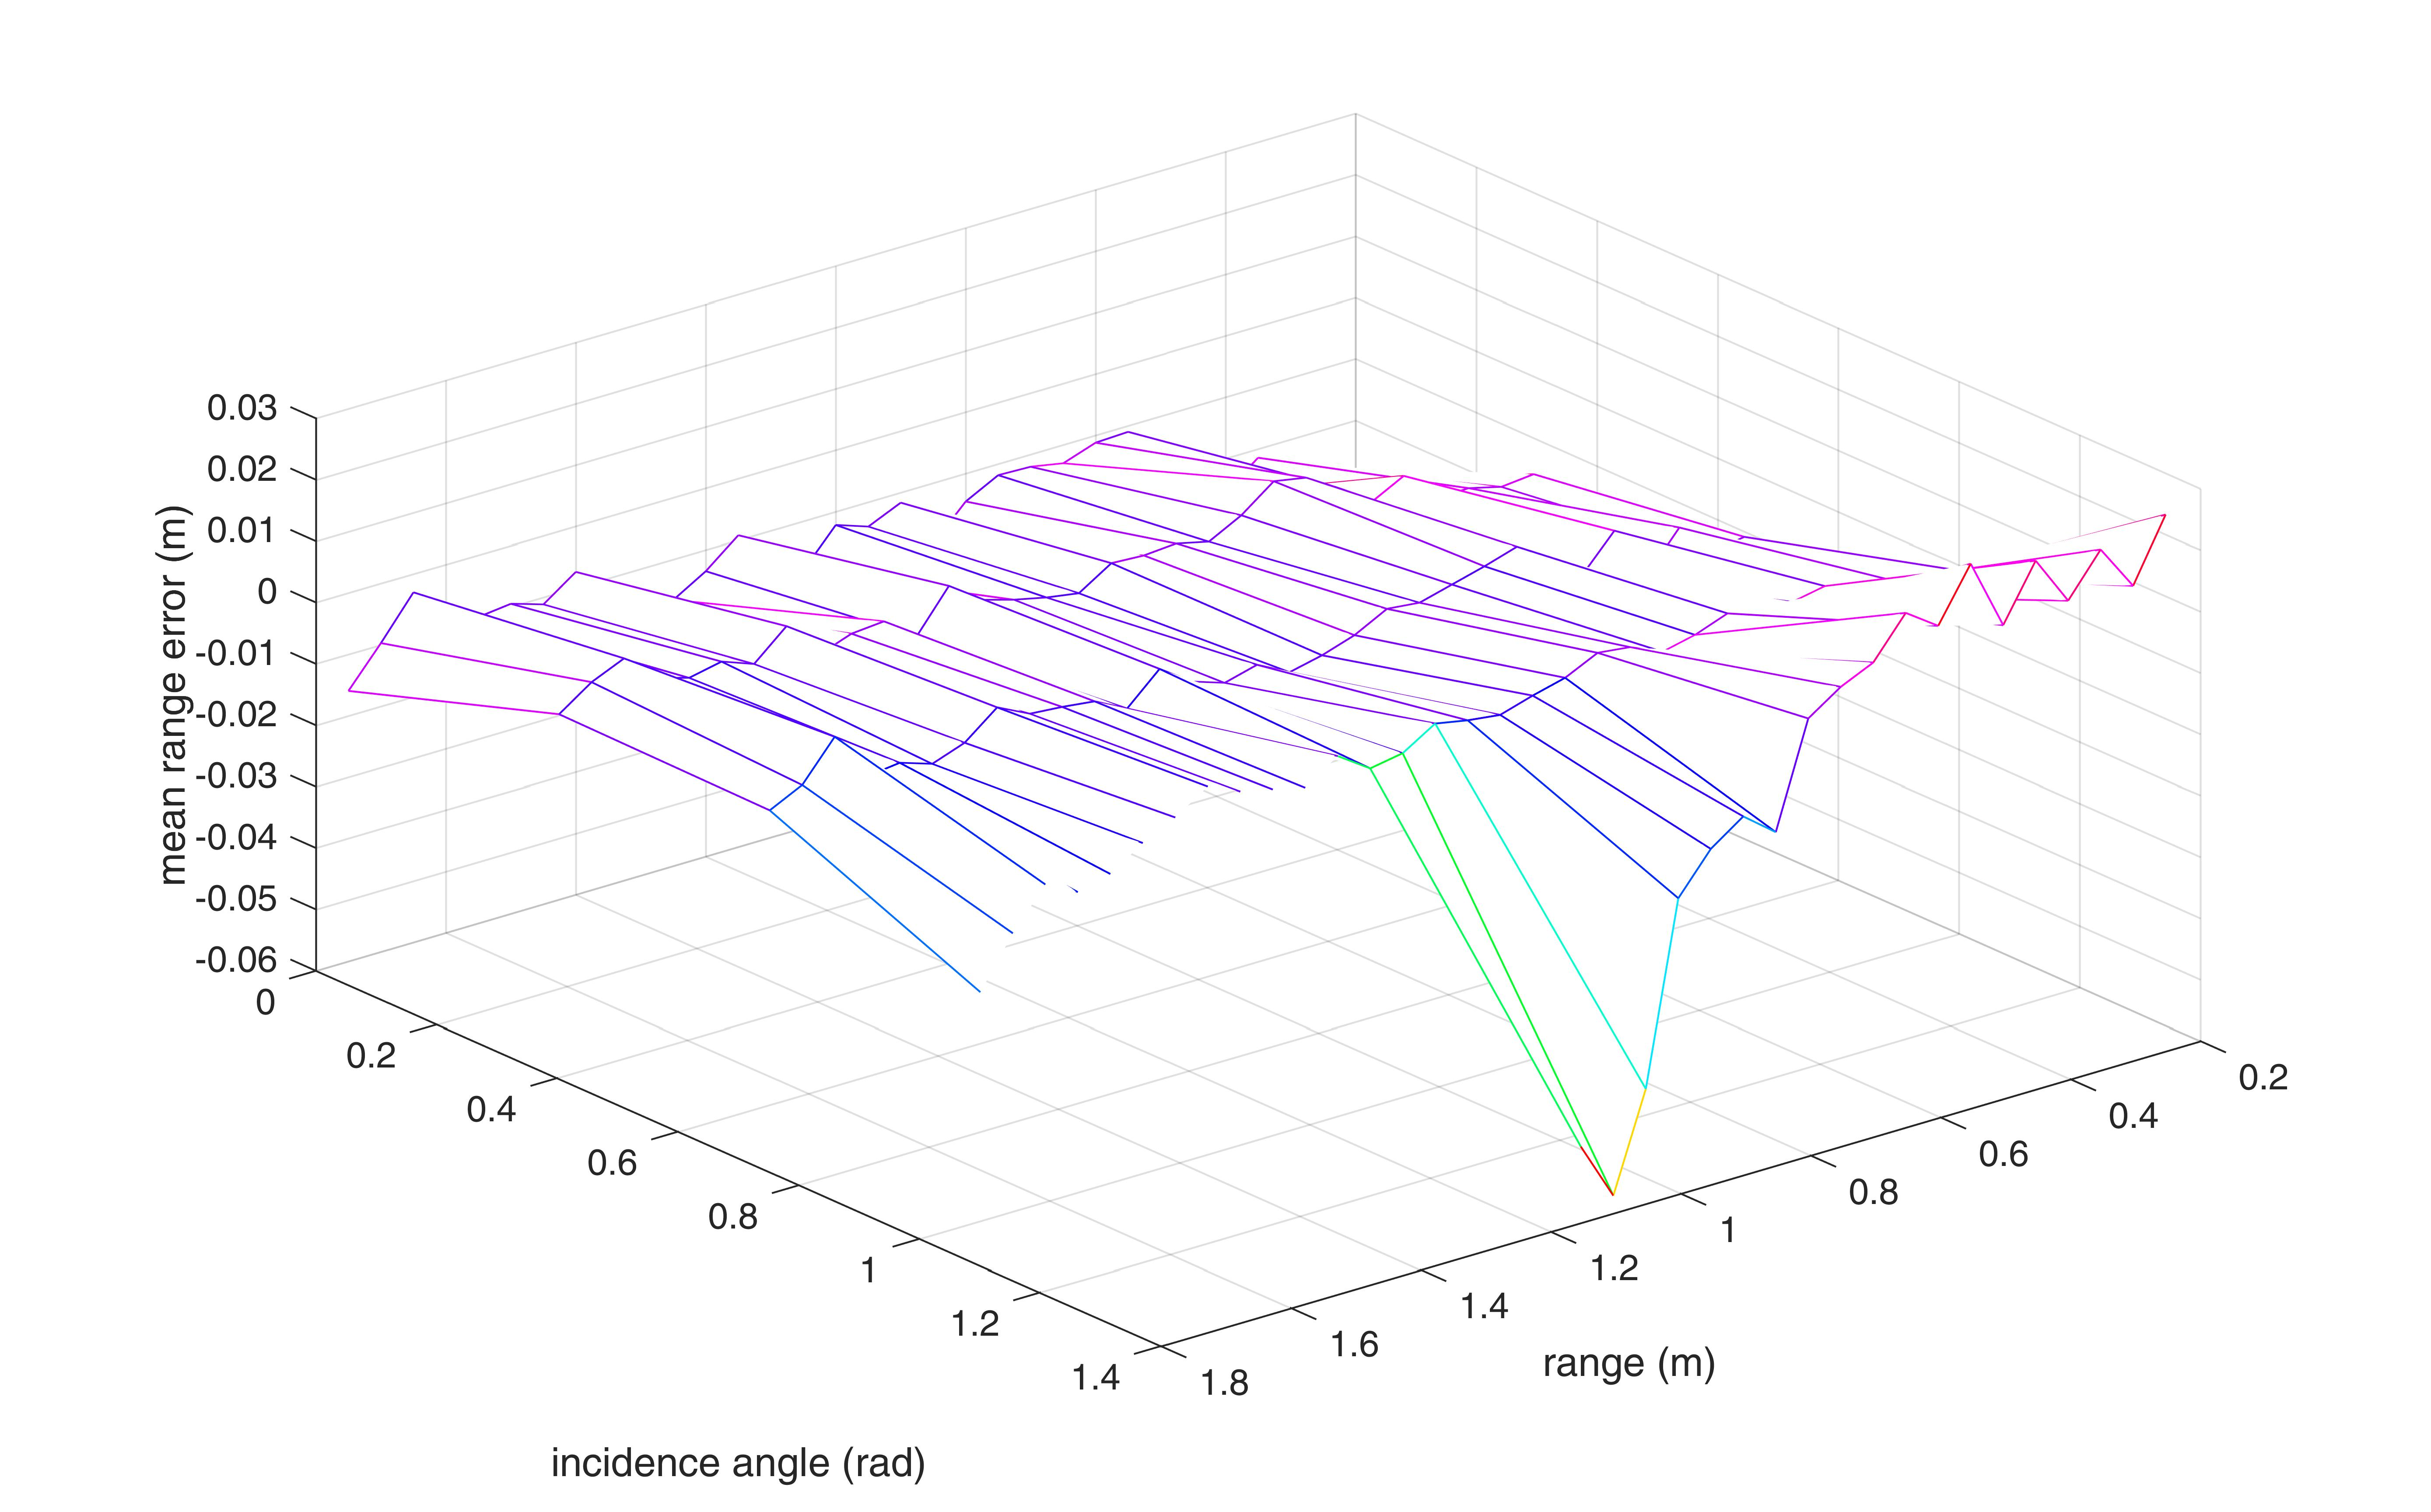
\includegraphics[width=1\textwidth,trim = 0mm 0mm 0mm 0mm,clip]{./Figures/noise_mean_range_error_removed_outliers}\vspace*{0ex}
		 \end{minipage}}
	  		\caption{mean range error vs $(r,\theta)$. (a) large error at high angles and range, (b) overall shape}
	  		\label{fig:mean_range_error}
		\end{figure}
		
		Std dev range error as function of (range,incidence angle) - Figure \ref{fig:stddev_range_error}		
		\begin{figure}
	  		\centering
	  		\subfigure[\label{fig:stddev_range_error_outliers}]{
	  		\begin{minipage}[b]{0.45\columnwidth}
    			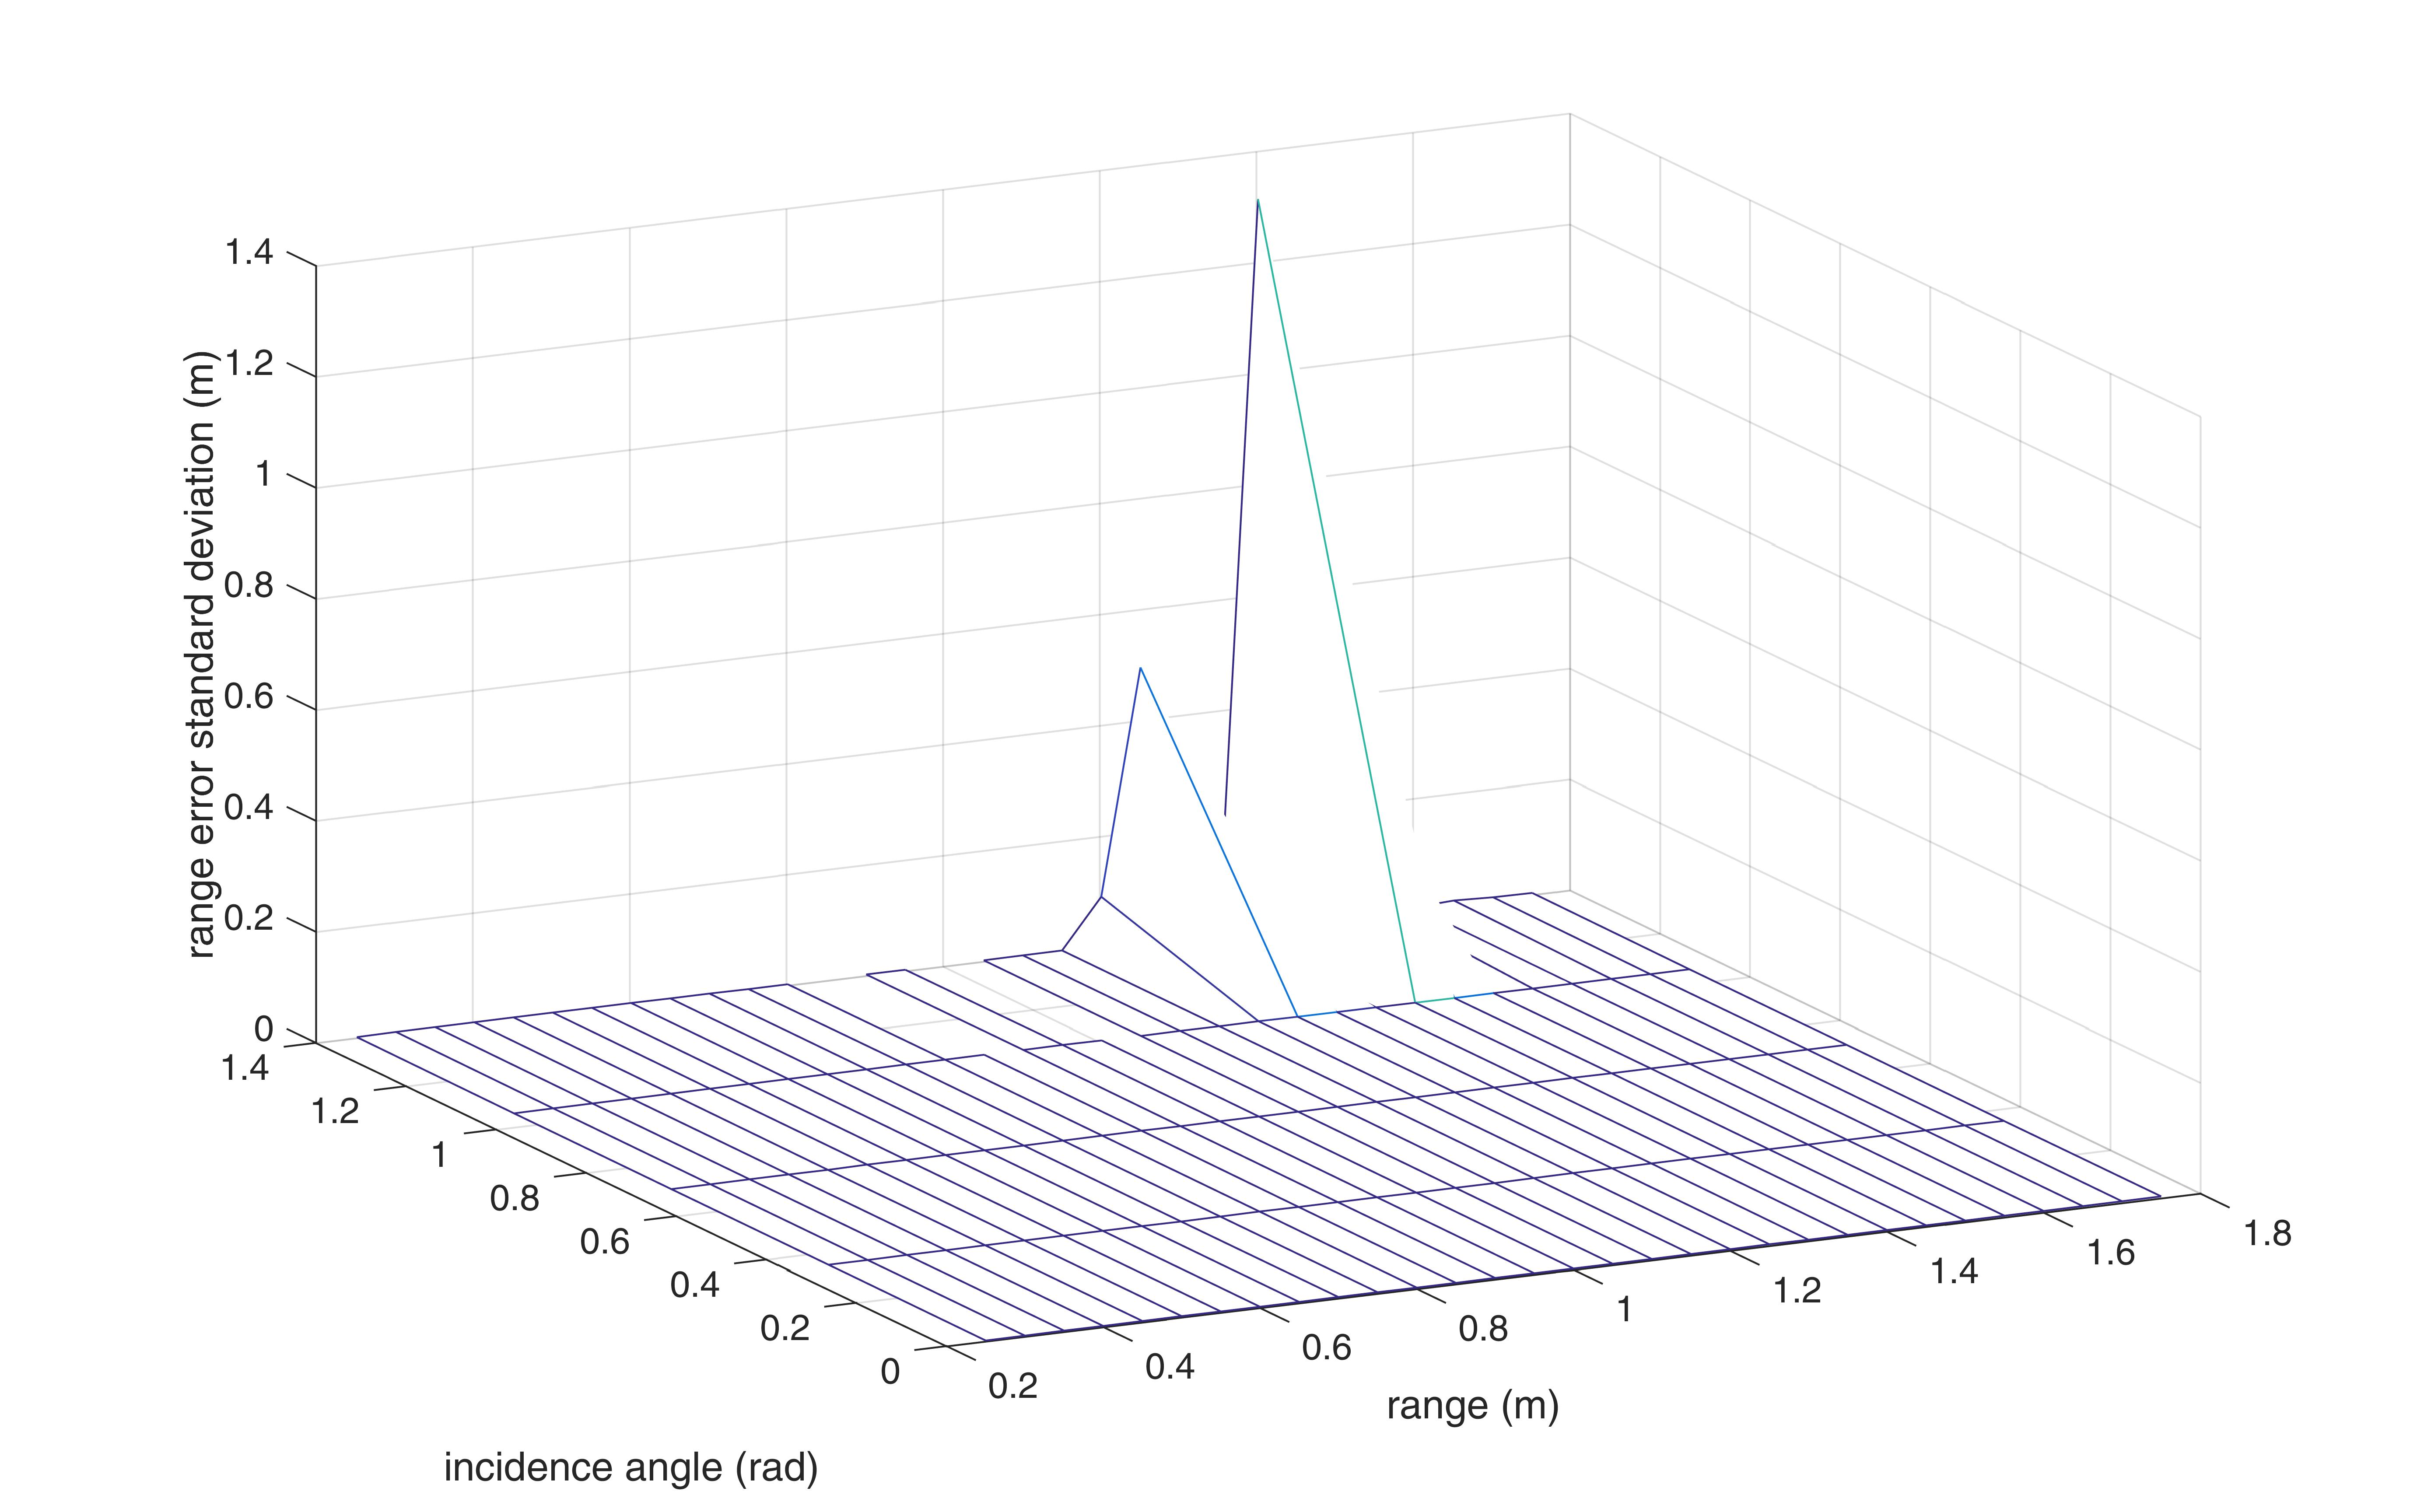
\includegraphics[width=1\textwidth,trim = 0mm 0mm 0mm 0mm,clip]{./Figures/noise_stddev_range_error}\vspace*{0ex}
	  		\end{minipage}}
	  		\subfigure[\label{fig:stddev_range_error_no_outliers}]{
	  		\begin{minipage}[b]{0.45\columnwidth}
    			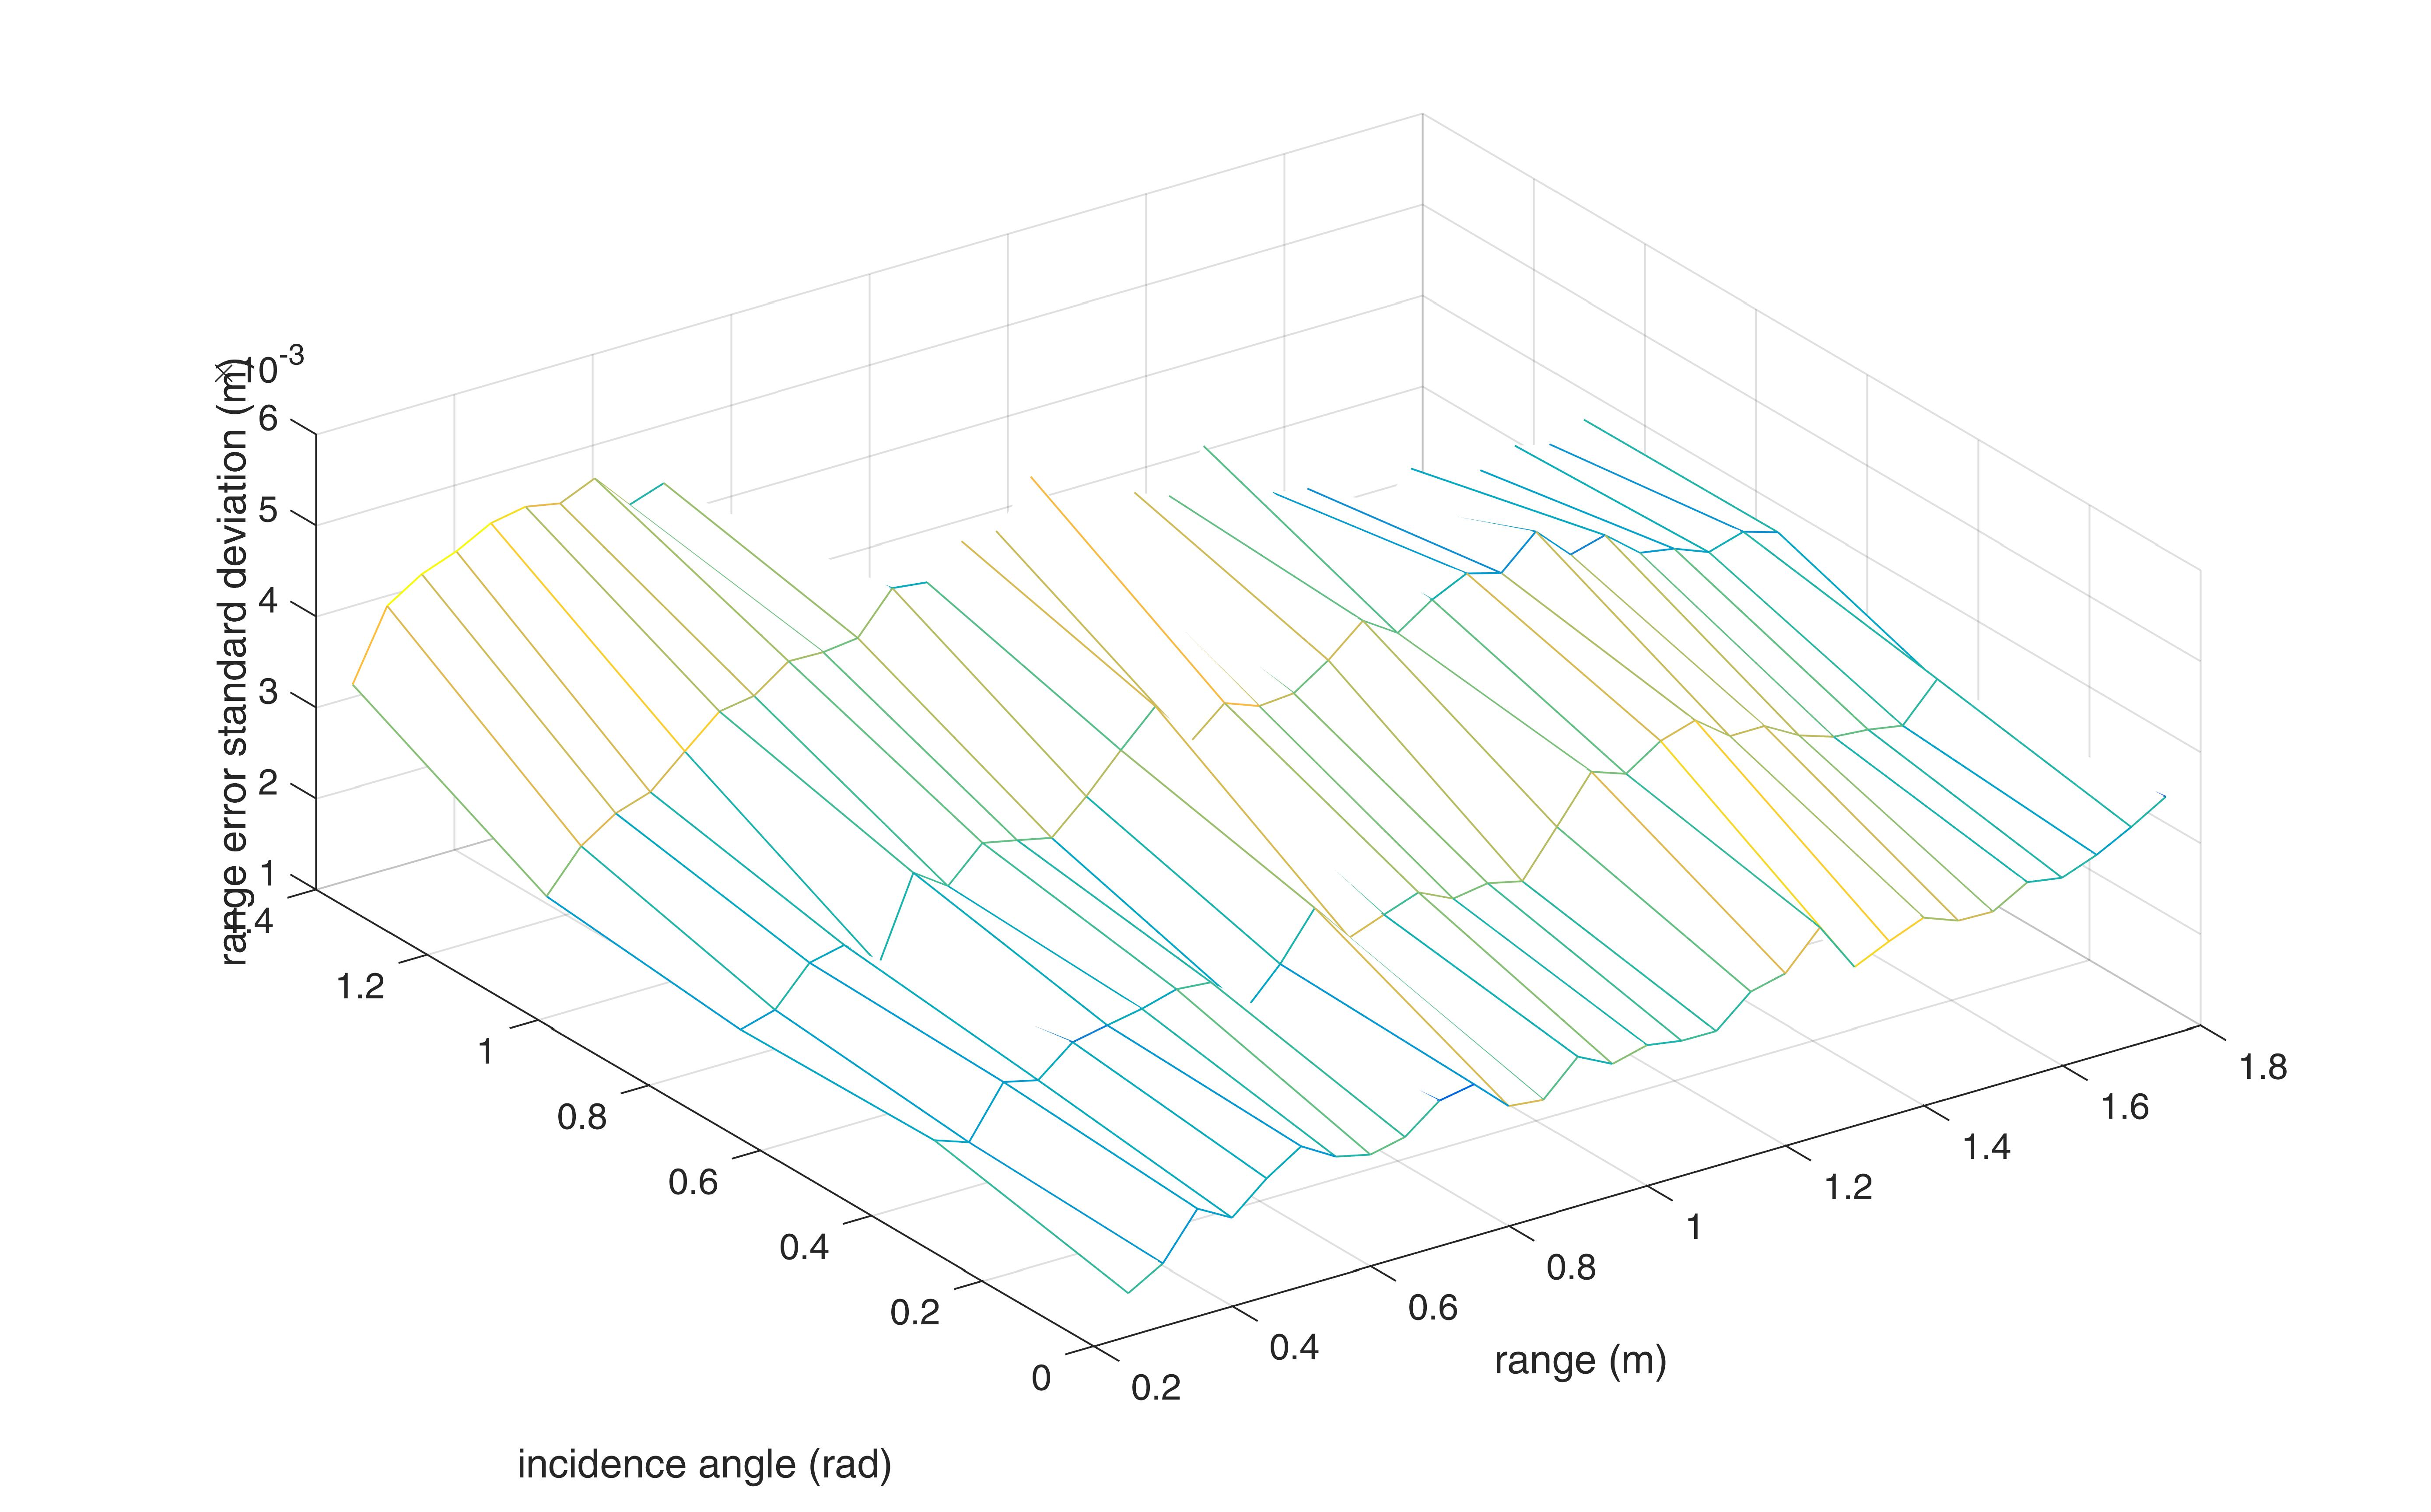
\includegraphics[width=1\textwidth,trim = 0mm 0mm 0mm 0mm,clip]{./Figures/noise_stddev_range_error_removed_outliers}\vspace*{0ex}
	 		 \end{minipage}}
	  		\caption{range error $\sigma$ vs $(r,\theta)$. (a) outliers/large std dev at high angles and range, (b) overall shape}
	  		\label{fig:stddev_range_error}
		\end{figure}
		
		Fitted 4th degree (in $x$ and $y$) polynomials to data points - Figure \ref{fig:surface_range_error}. INCLUDE FIT DATA
		\begin{figure}
	  		\centering
	  		\subfigure[\label{fig:surface_mean_range}]{
	  		\begin{minipage}[b]{0.45\columnwidth}
    			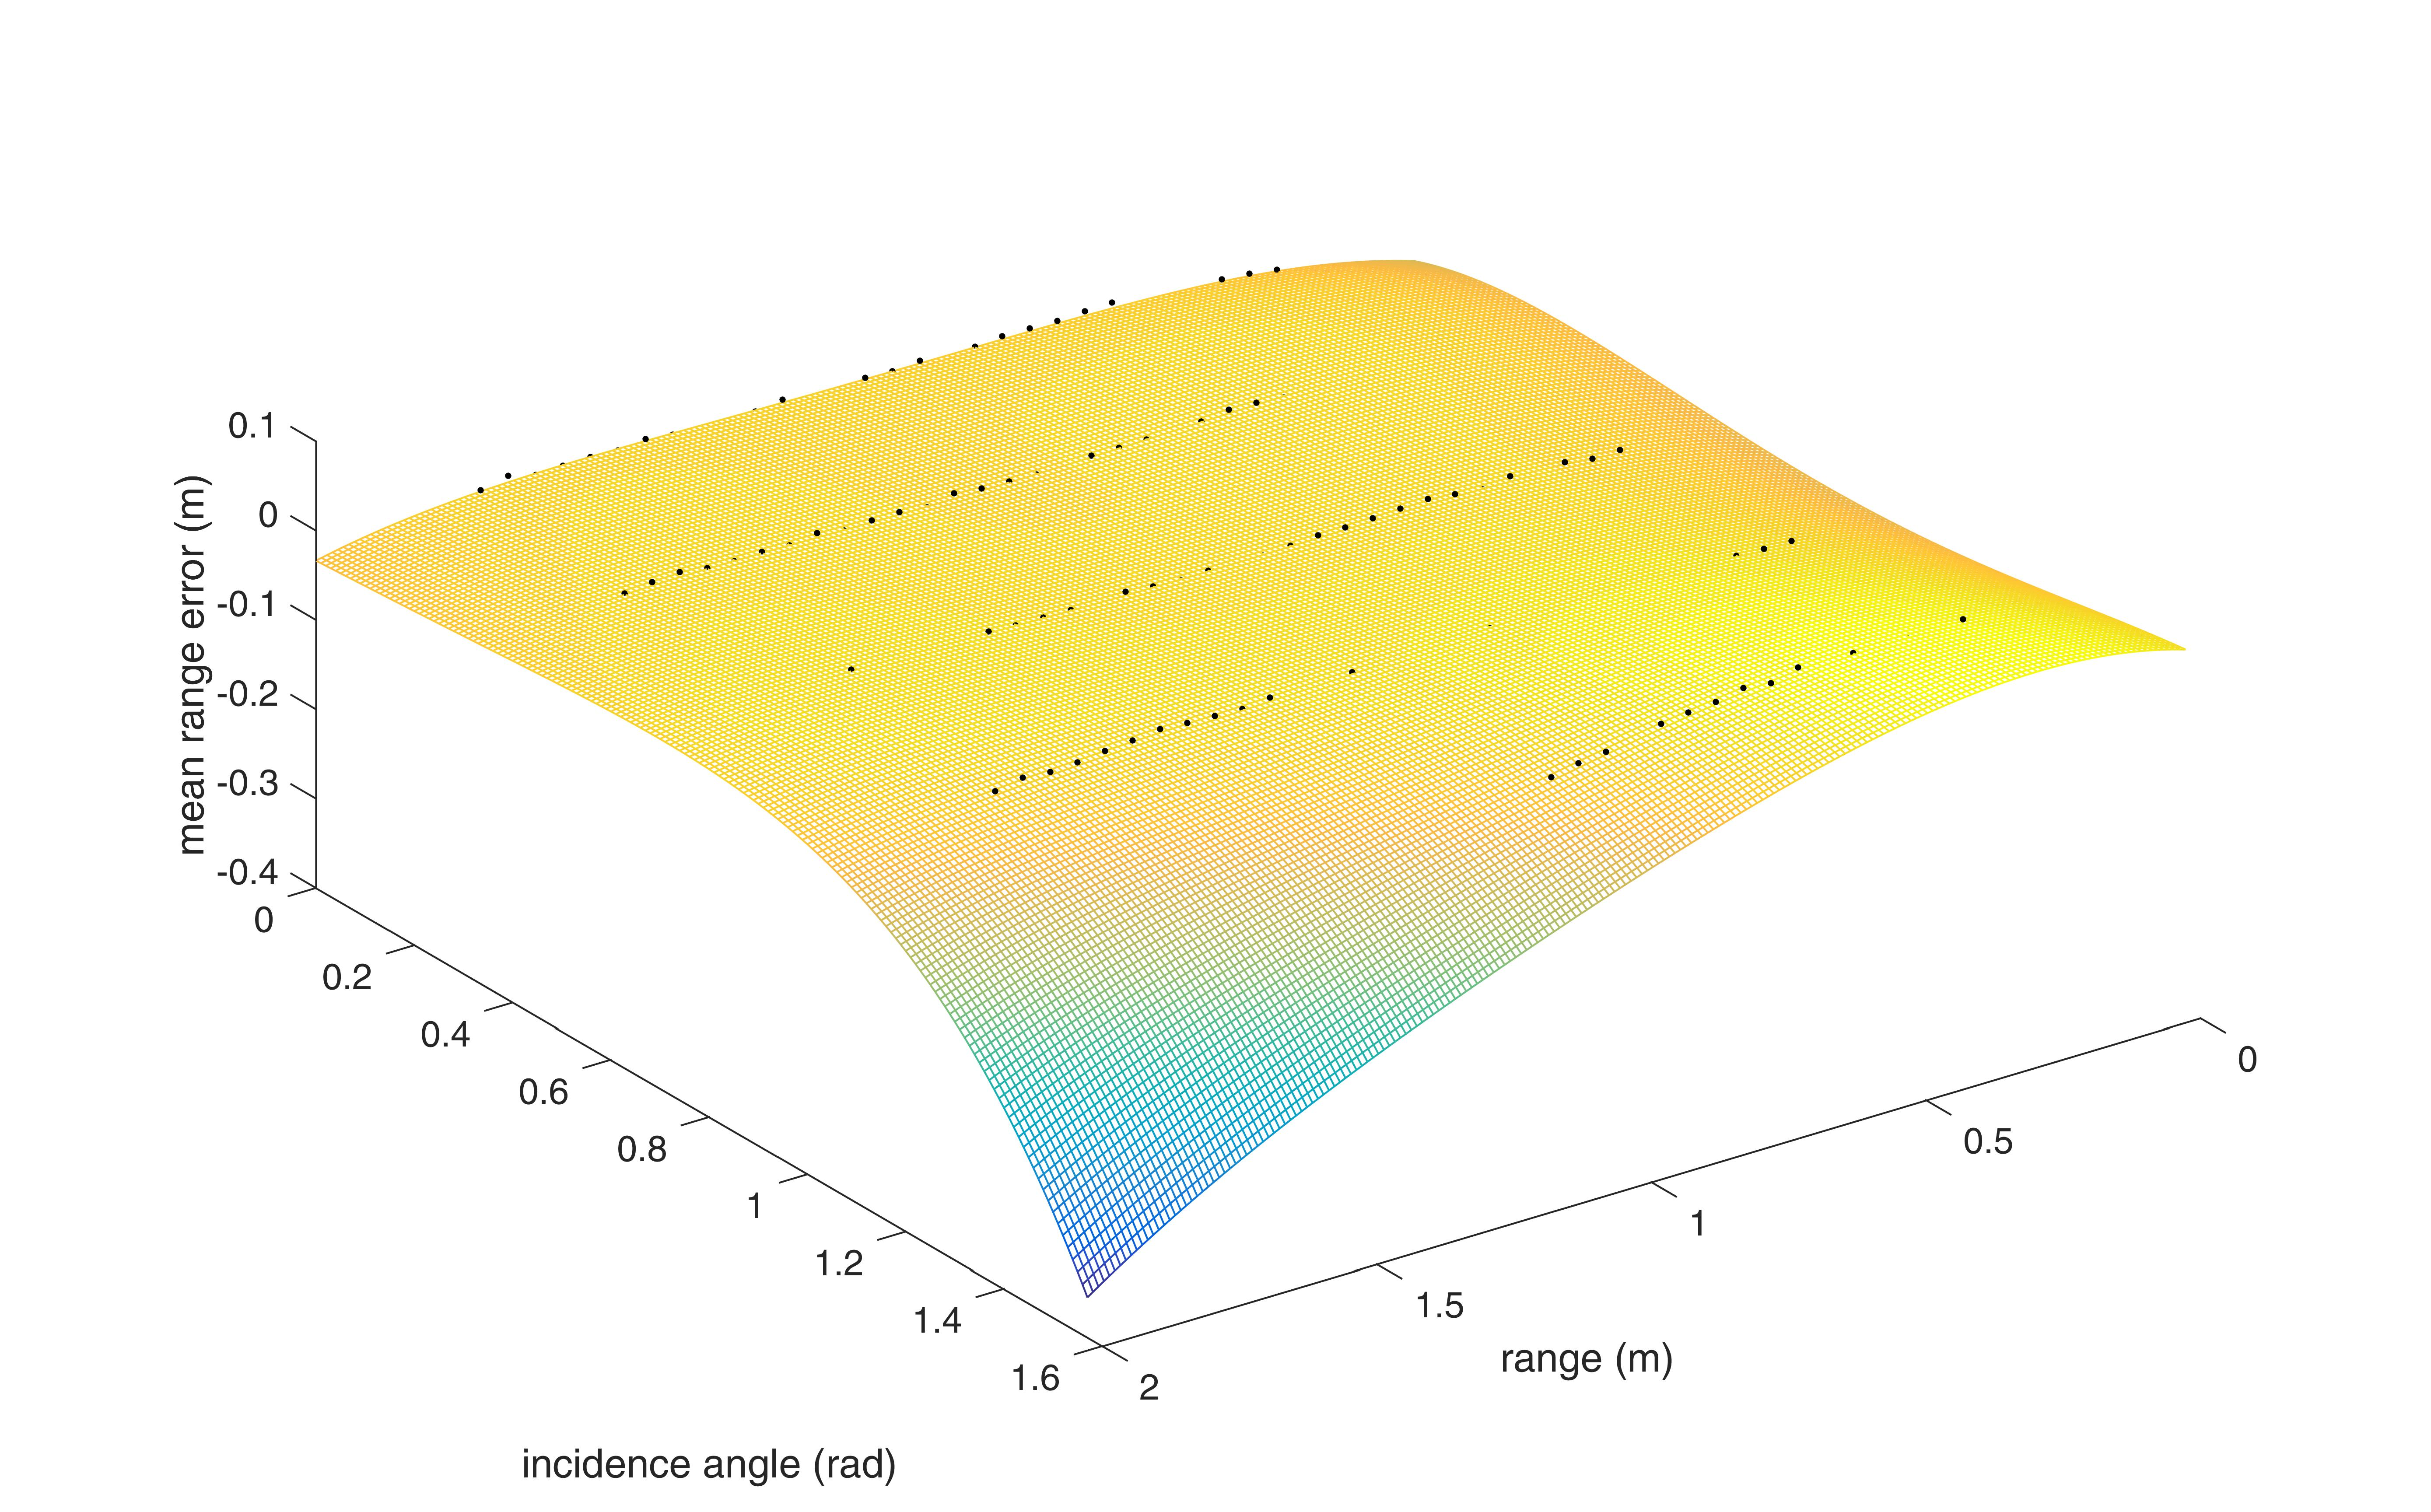
\includegraphics[width=1\textwidth,trim = 0mm 0mm 0mm 0mm,clip]{./Figures/surface_mean_range_error}\vspace*{0ex}
	  		\end{minipage}}
	  		\subfigure[\label{fig:surface_stddev_range}]{
	  		\begin{minipage}[b]{0.45\columnwidth}
    			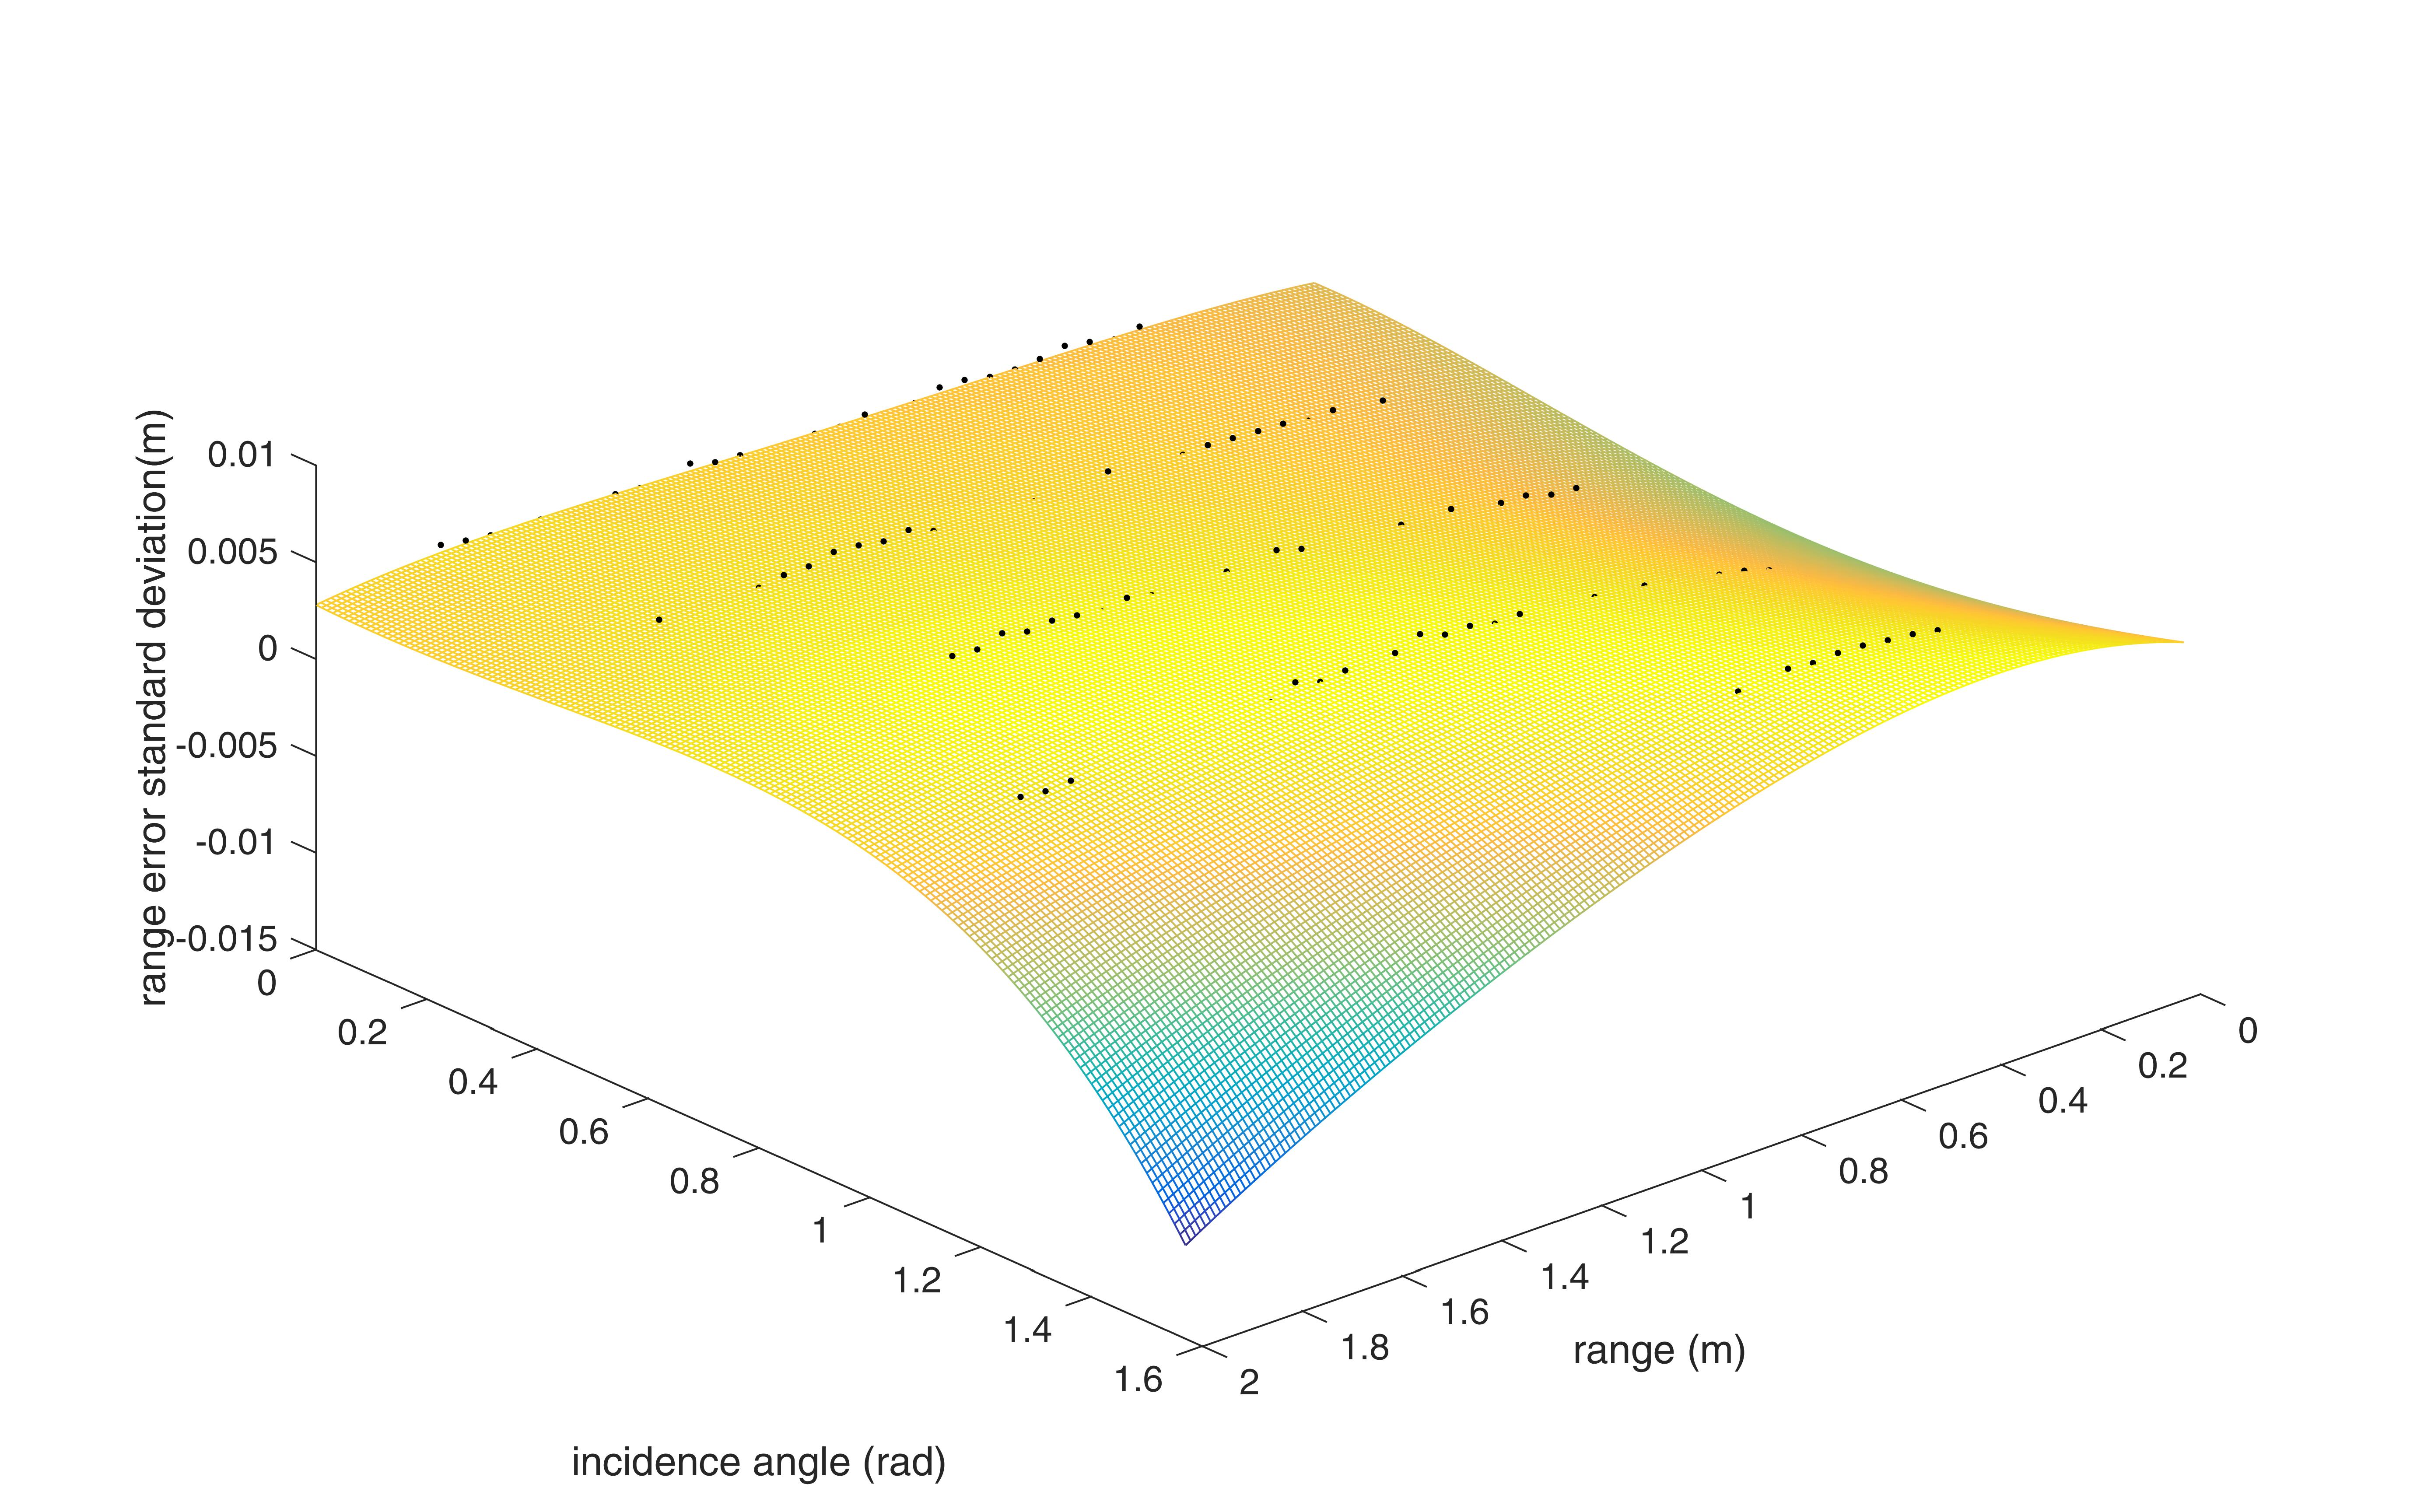
\includegraphics[width=1\textwidth,trim = 0mm 0mm 0mm 0mm,clip]{./Figures/surface_stddev_range_error}\vspace*{0ex}
		 \end{minipage}}
	  		\caption{polynomials fitted to range error mean \& standard deviation data points to model noise}
	  		\label{fig:surface_range_error}
		\end{figure}
		
		Noise Model:\\
		\begin{equation}
			r_{error} = r + \mathcal{N}(\mu,\sigma)
		\end{equation}	
		
		\begin{equation}
			\begin{aligned}
				\mu = & a_{00} + a_{10}r + a_{01}\theta + a_{20}r^2 + a_{11}r\theta + a_{02}\theta^2\\
				      & + a_{30}r^3 + a_{21}r^2\theta + a_{12}r\theta^2 + a_{03}\theta^3 + a_{40}r^4 \\ 
				      & + a_{31}r^3\theta + a_{22}r^2\theta^2 + a_{13}r\theta^3 + a_{04}\theta^4
			\end{aligned}		
		\end{equation}
		\begin{equation}
			\begin{aligned}
				\sigma = & b_{00} + b_{10}r + b_{01}\theta + b_{20}r^2 + b_{11}r\theta + b_{02}\theta^2\\
			         	 & + b_{30}r^3 + b_{21}r^2\theta + b_{12}r\theta^2 + b_{03}\theta^3 + a_{40}r^4 \\ 
			         	 & + b_{31}r^3\theta + b_{22}r^2\theta^2 + b_{13}r\theta^3 + b_{04}\theta^4
			\end{aligned}
		\end{equation}
		
		*outliers ignored in model. if angle $>$ 75 deg and range $>$ 0.8m, range measurement = NaN. EXPLANATION: as angle increases, measured range becomes less than ground truth - due to beam width. part of beam hits part of object that is closer due to angle. However, as angle increases further, not enough light returns to make measurements. At high ranges and angles, measurement is not of object, but due to reflections that take much longer. Measurement ends up being near maximum range or even INF. Instead, will set as NaN - no value returned.
		
		Coefficients in tables \ref{tab:noise_a} and \ref{tab:noise_b}
		\begin{table}[h!]
  \centering
  \caption{$a_{ij}$ coefficients}
  \label{tab:noise_a}
  \begin{tabular}{c| c c c c c}
     	  & $j_0$ 	 & $j_1$   & $j_2$ 	 & $j_3$   & $j_4$ \\
    \hline
   	$i_0$ & -0.06529 & 0.2126  & -0.533	 & 0.4629  & -0.1223 \\
   	$i_1$ & 0.2024   & -0.1906 & 0.4006	 & -0.1791 & 0 \\
   	$i_2$ & -0.3074  & 0.0228  & -0.0716 & 0 	   & 0 \\
   	$i_3$ & 0.2053   & 0.01455 & 0 		 & 0 	   & 0 \\
   	$i_4$ & -0.04912 & 0 	   & 0 		 & 0 	   & 0 \\
  \end{tabular}
\end{table}



		\begin{table}[h!]
  \centering
  \caption{$b_{ij}$ coefficients}
  \label{tab:noise_b}
  \begin{tabular}{c| c c c c c}
		  & $j_0$ 	  & $j_1$    & $j_2$ 	  & $j_3$	  & $j_4$ \\
	\hline
	$i_0$ & 0.001242  & 0.2126	 & -0.01128	  & 0.01162	  & -0.002746 \\
	$i_1$ & 0.00352   & 0.006146 & 0.01021	  & -0.007316 & 0 \\
	$i_2$ & -0.005138 & -0.00626 & -0.0005068 & 0 		  & 0 \\
	$i_3$ & 0.004067  & 0.001337 & 0 		  & 0 		  & 0 \\
	$i_4$ & -0.001092 & 0 		 & 0 		  & 0 		  & 0 \\
  \end{tabular}
\end{table}





		\textbf{Surface noise:}
		random walk model\\
		have observed error mostly independent of range and angle - seems to be some compensation performed by sensor to get straight lines - range across smooth surfaces that should be appear as straight lines varies regularly.
		Could be surface properties of objects, though error is larger than expected in this case.
		Profile of error sinusoidal (regular-ish peaks and valleys), peaks = 5mm deep \& 50mm wide approximately
		
		add random walk to each scan
		\begin{equation}
			error = a\sum_{n = 1}^{n_{Steps}}-1 + 2\:\left \lfloor{\mathcal{R}}\right \rfloor 
		\end{equation} 
		where $\mathcal{R}$ is a random variable following a uniform distribution on [0,1]
		Doesn't work too well over long surfaces (~1m) - can get too large sometimes, but fits measured data for small objects like cube
		
		Figure \ref{fig:surface_noise}: comparison of simulated \& measured surface noise:
		\begin{figure}
	  		\centering
	  		\subfigure[\label{fig:measured_surface_noise}]{
	  		\begin{minipage}[b]{0.45\columnwidth}
    			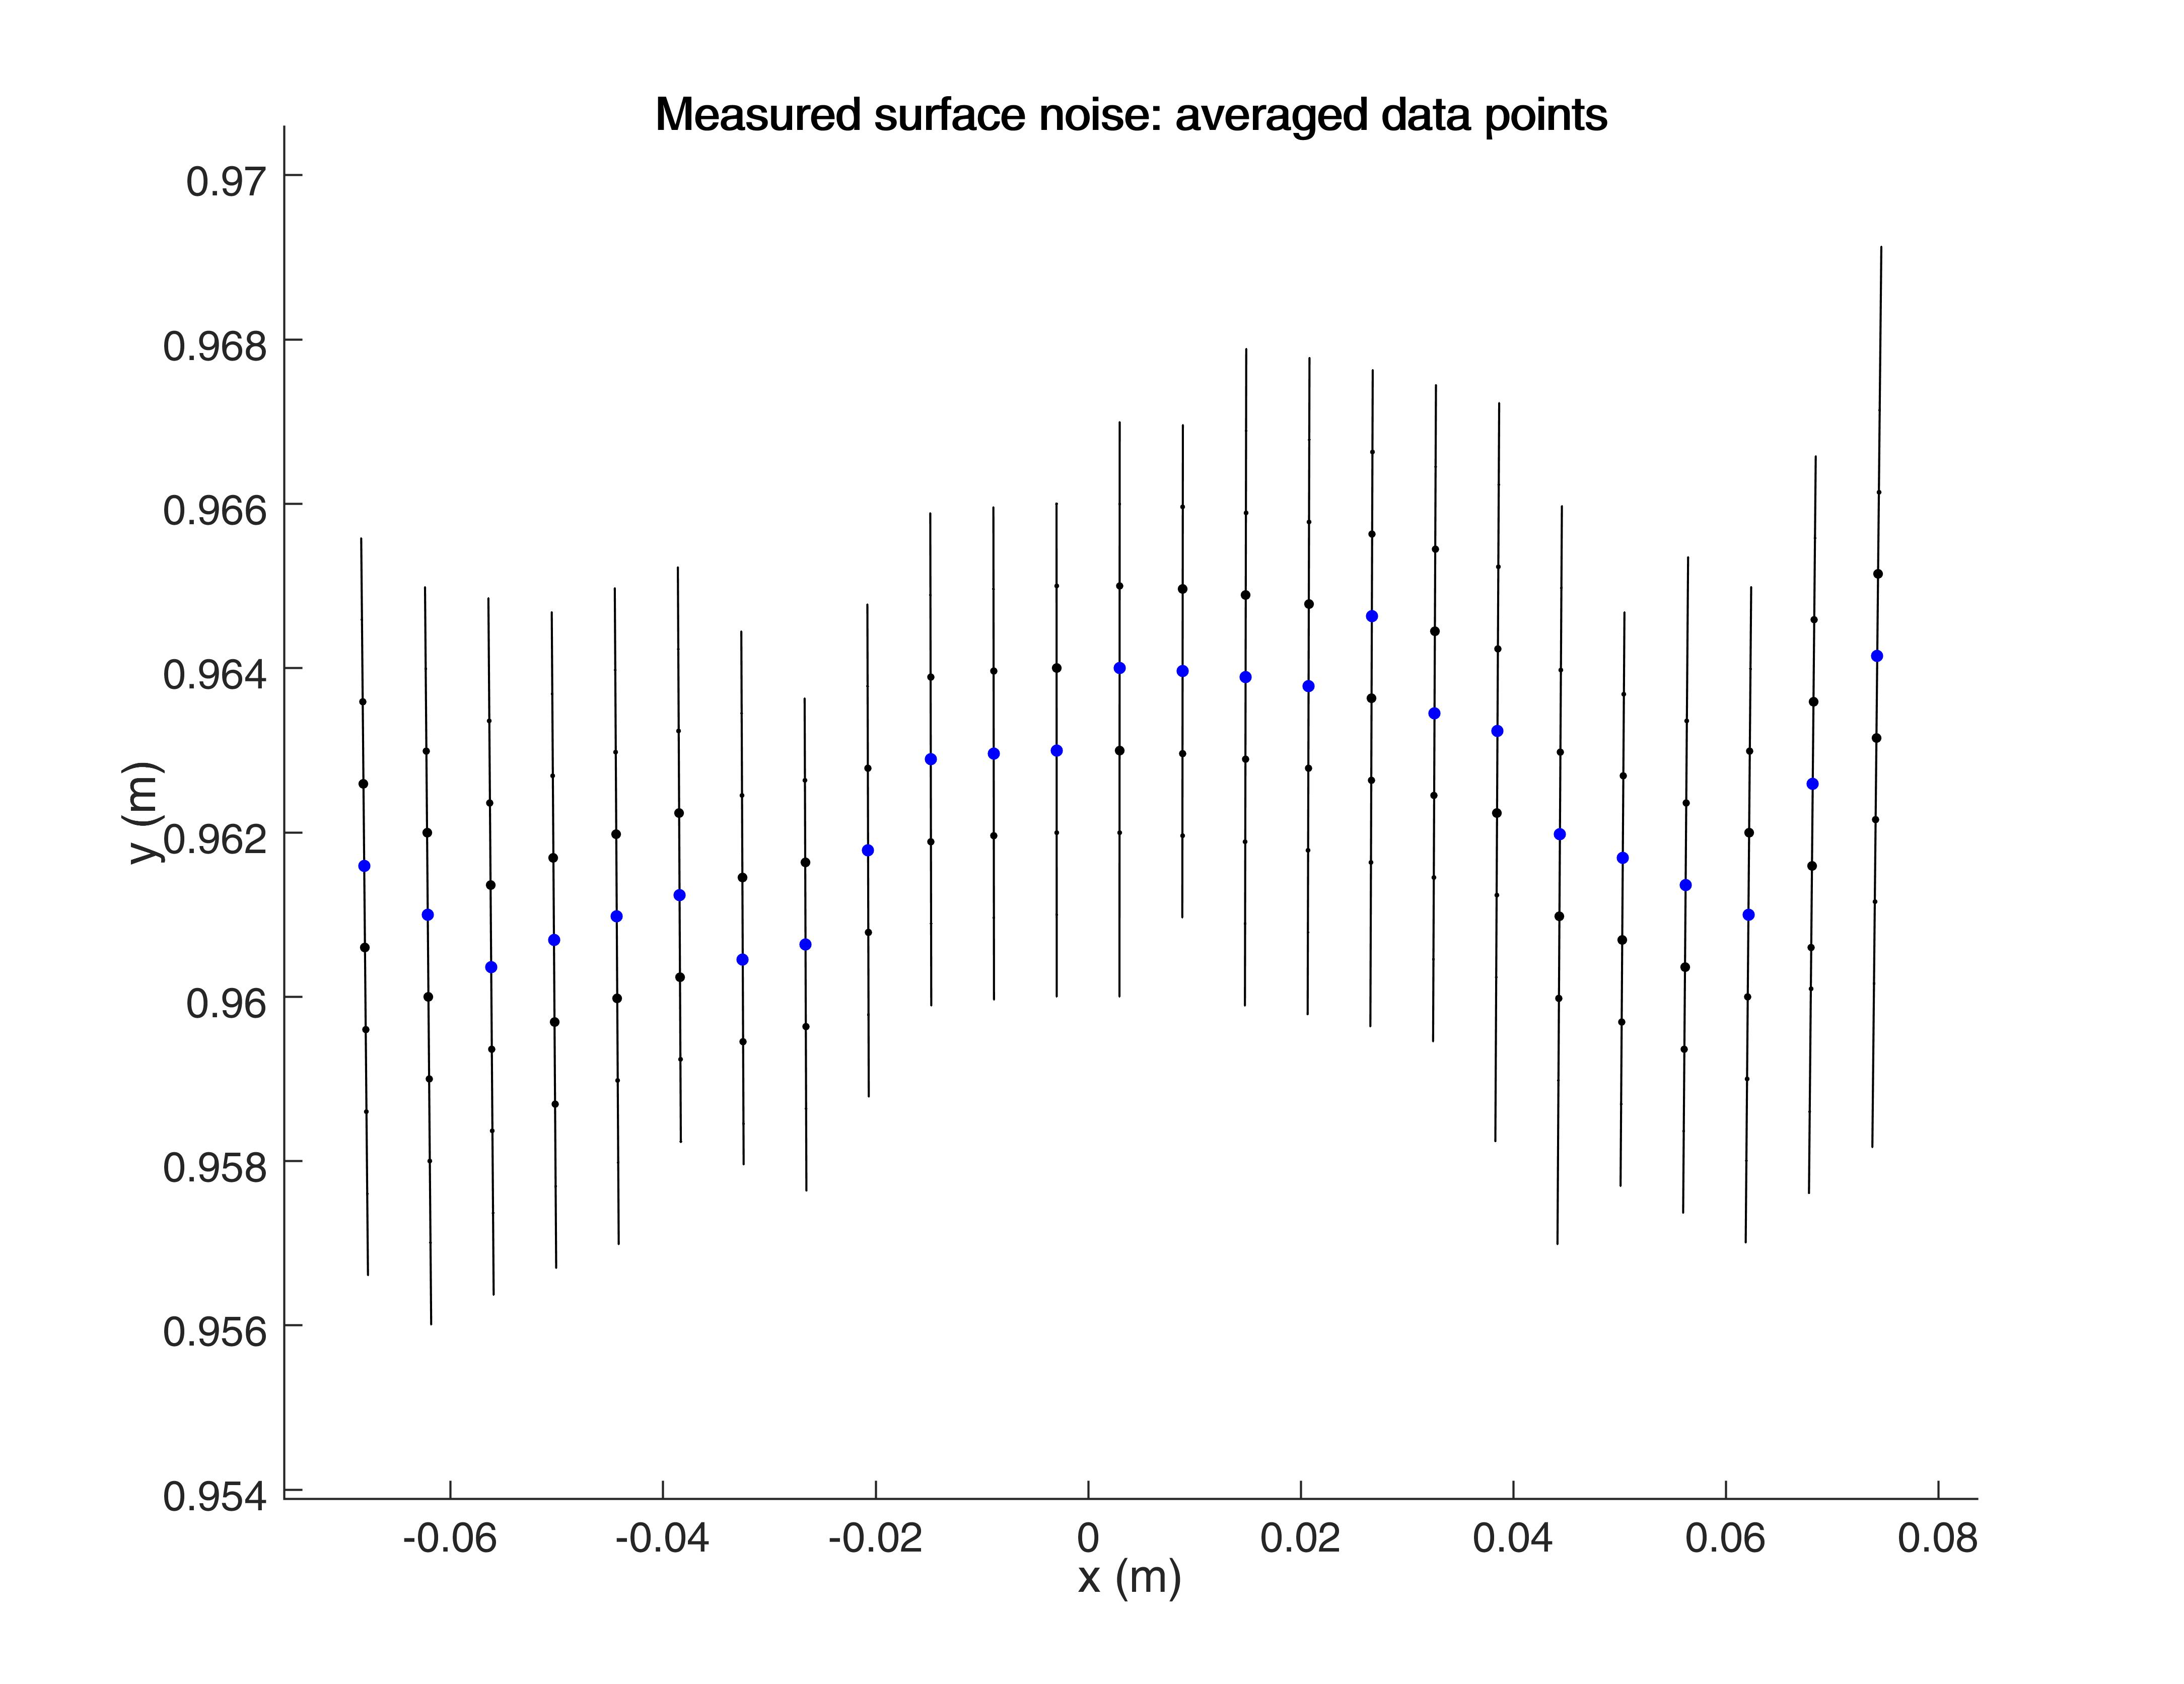
\includegraphics[width=1\textwidth,trim = 0mm 0mm 0mm 0mm,clip]{./Figures/measured_surface_noise}\vspace*{0ex}
	  		\end{minipage}}
	  		\subfigure[\label{fig:simulated_surface_noise}]{
	  		\begin{minipage}[b]{0.45\columnwidth}
    			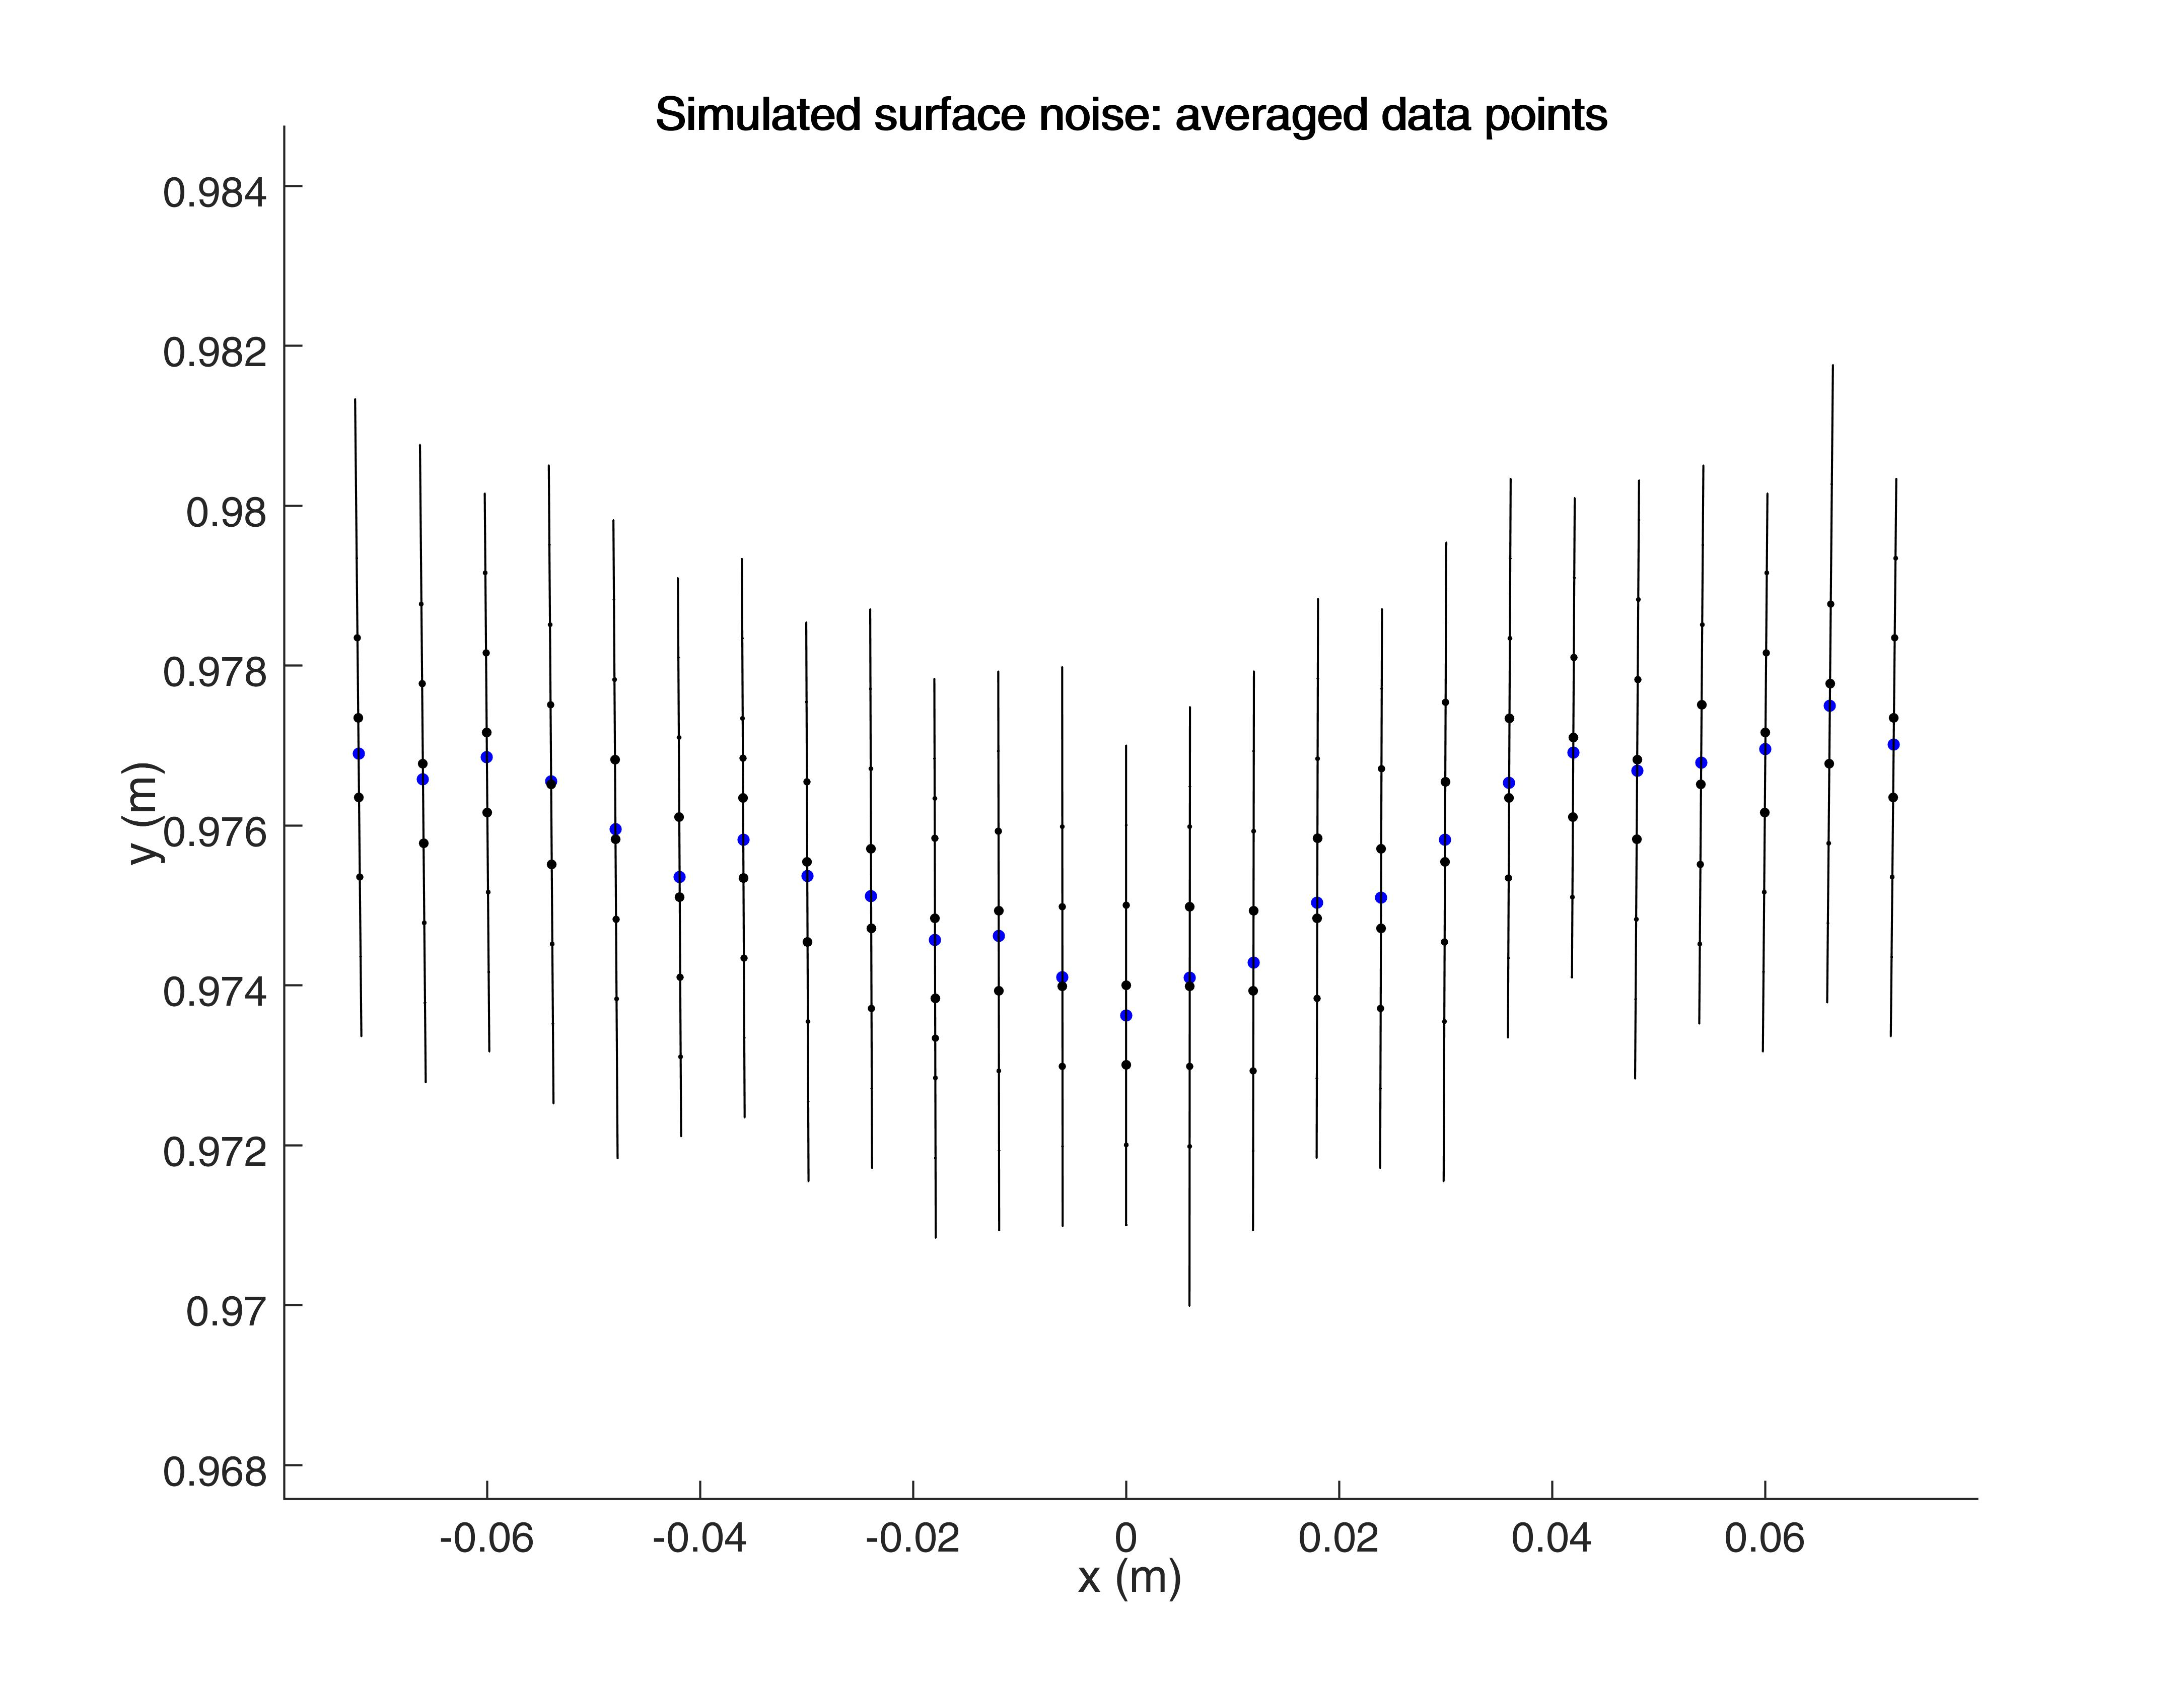
\includegraphics[width=1\textwidth,trim = 0mm 0mm 0mm 0mm,clip]{./Figures/simulated_surface_noise}\vspace*{0ex}
 			\end{minipage}}
	  		\caption{Comparision of (a) measured and (b) simulated surface noise}
	  		\label{fig:surface_noise}
		\end{figure}

\section{Testing Data Collection}
	\subsection{Setup}
		physical setup\\
		configurations/motions: \\
			-stationary\\
			-rotating\\
			-translating\\
			(all above with 1,2,3 faces visible to sensor)
					
		arm forward kinematics $\rightarrow$ cube pose\\
		estimate sensor angle with horizontal with wall calibration data		
		
	\subsection{Results}
		observer performance

